\documentclass[final,3p,times,twocolumn]{elsarticle}

\usepackage[T1]{fontenc}
\usepackage{amsmath,amssymb}
\usepackage{graphicx}
\usepackage{float}
\usepackage{placeins}
\usepackage{dblfloatfix}
\usepackage[font=small,labelfont=bf]{caption}
\usepackage{microtype}
\usepackage{listings}
\usepackage{needspace}
\usepackage{tabularx}
\usepackage[hidelinks]{hyperref}

\flushbottom
\emergencystretch=1em

\lstset{
  basicstyle=\ttfamily\footnotesize,
  breaklines=true,
  breakatwhitespace=false,
  columns=fullflexible,
  keepspaces=true
}

\renewcommand{\topfraction}{0.9}
\renewcommand{\bottomfraction}{0.8}
\renewcommand{\textfraction}{0.08}
\renewcommand{\floatpagefraction}{0.85}
\setcounter{topnumber}{3}
\setcounter{bottomnumber}{2}
\setcounter{totalnumber}{4}

\setlength{\textfloatsep}{6pt plus 1pt minus 2pt}
\setlength{\floatsep}{4pt plus 1pt minus 1pt}
\setlength{\intextsep}{6pt plus 1pt minus 2pt}
\setlength{\dbltextfloatsep}{6pt plus 1pt minus 2pt}
\setlength{\dblfloatsep}{4pt plus 1pt minus 1pt}
\captionsetup{skip=3pt,justification=raggedright,singlelinecheck=false}

\newif\ifwithpaths
\withpathsfalse
\DeclareRobustCommand{\pathnote}[1]{\ifwithpaths\textit{ [source: \nolinkurl{#1}]}\fi}

\journal{MPhil in Scientific Computing}


\begin{document}

\begin{frontmatter}

\title{Adaptive Mesh Refinement and Parallelisation for the Compressible Euler Equations Using AMReX}

\author{Portfolio version}

\begin{abstract}
This report evaluates whether block-structured adaptive mesh refinement (AMR) in AMReX preserves credible solution behaviour for the compressible Euler equations while reducing time-to-solution under matched finest-spacing comparisons. The solver uses an HLL approximate Riemann solver with Davis wave-speed bounds for spatial fluxes, MUSCL reconstruction with a componentwise minmod limiter, and SSPRK2 (Heun's method) time integration. It enforces positivity with density/pressure floors during reconstruction and a per-stage energy reset when the pressure floor activates (strictly non-conservative only in cells where the reset activates).

The evidence is organised around three questions: shock-dominated refinement behaviour in one dimension, orientation consistency in two dimensions, and runtime decomposition between AMR localisation and MPI strong scaling on a single node. On discontinuity-dominated tests, mean observed orders are first-order-like ($\approx 0.5$--$0.6$), while a supplementary smooth Gaussian test gives near-second-order density convergence with $L_1$ orders 1.79 and 1.84. For the quadrant benchmark, AMR reduces single-core wall-clock runtime by $4.32\times$ at $N_\mathrm{eff}=1536$ and $14.67\times$ at $N_\mathrm{eff}=3072$. A repeated AMR+MPI configuration at $p=4$ reduces time-to-solution by $33.33\times$ versus the repeated uniform $N=3072$ serial baseline, while the fastest single measured run reaches $33.61\times$; gains flatten beyond about four ranks on this node. The stricter full-field quadrant diagnostic, however, does not support a blanket matched-spacing AMR accuracy advantage. The evidence therefore supports strong single-node performance gains and credible shock-oriented behaviour, but not a general claim of superior matched-spacing AMR accuracy or multilevel smooth-order recovery.
\end{abstract}

\end{frontmatter}


\section{Introduction}
\label{sec:introduction}

The compressible Euler equations are a standard model for inviscid gas dynamics. Toro's text is used here as the main benchmark reference for shock-capturing finite-volume methods \cite{toro2009}. In conservative form, the two-dimensional system is
\begin{equation}
\partial_t \mathbf{U} + \nabla\cdot\mathbf{F}(\mathbf{U})=\mathbf{0},
\end{equation}
where $\mathbf{U}=(\rho,\rho u,\rho v,E)^\mathsf{T}$ is the conservative state vector, $\rho$ is density, $(u,v)$ are velocity components, and $E$ is total energy density. Pressure is recovered from the ideal-gas closure
\begin{equation}
p=(\gamma-1)\left(E-\tfrac{1}{2}\rho(u^2+v^2)\right),
\end{equation}
with $\gamma=1.4$ in all runs reported here.

Discontinuous initial data produce shocks, contacts, and rarefactions, so the method requires robust conservative fluxes near sharp discontinuities. Uniform two-dimensional runs also become expensive under refinement because both the cell count and the step count increase. Adaptive mesh refinement (AMR) helps by placing fine cells near sharp features while keeping smooth regions coarse \cite{berger1989}. AMReX provides the block-structured AMR framework used in this study \cite{AMReX_JOSS,AMReX_IJHPCA1,amrexdocs}. The question is therefore not simply whether AMR can be faster, but which accuracy and performance claims survive matched finest-spacing comparisons under fixed baselines.

Task 1 uses Toro's one-dimensional Riemann problems to check refinement trends at matched finest spacing. Task 2 extends the same setup to two dimensions and checks orientation consistency for axis-aligned $x$-split and $y$-split cases before stressing the solver with diagonal discontinuities. Task 3 measures runtime on a two-dimensional quadrant benchmark and asks how AMR localisation and MPI strong scaling combine on a single node under fixed timing controls.

The analysis is split into discretisation behaviour under refinement, orientation consistency under rotation, and runtime decomposition into algorithmic localisation and MPI scaling, because similar headline speed-ups can arise from different mechanisms. Throughout, ``matched finest spacing'' means that a uniform run and an AMR run are compared at the same finest-level cell size; the corresponding uniform grid size is denoted the effective resolution $N_\mathrm{eff}$. Accuracy claims use exact references or symmetry residuals; performance claims use fixed runtime controls on one machine.

HLL is less contact-sharp than contact-resolving alternatives, but it is robust on strong shocks and adequate for the directional checks used here.

Figure~\ref{fig:intro_amr_localisation} illustrates the localisation mechanism on Toro Test 1 at matched effective resolution. Refined bands cluster near wave features, while smooth regions remain at coarse levels. This is the core mechanism quantified later through error ratios and timing decomposition.

\begin{figure}[!tbp]
    \centering
    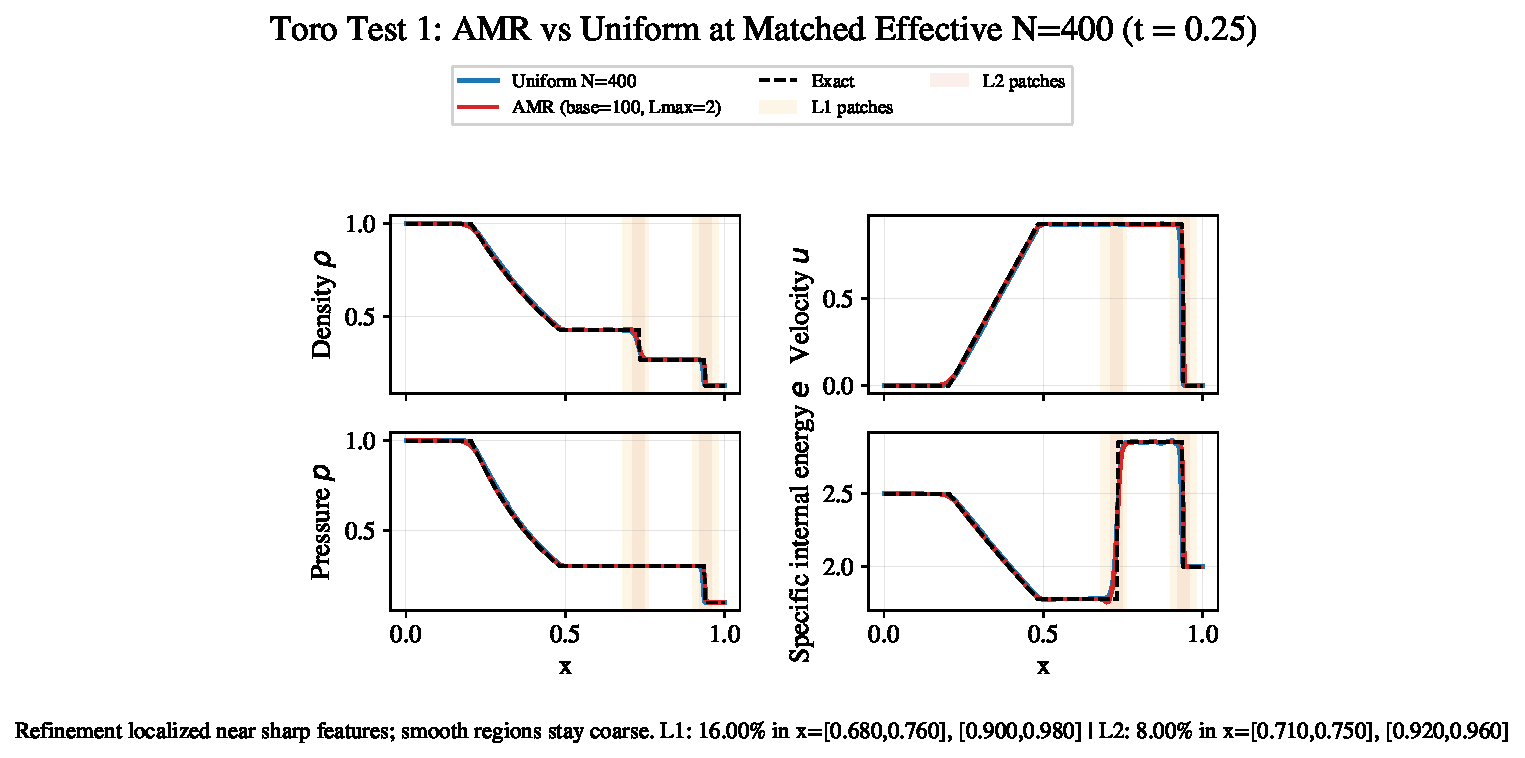
\includegraphics[width=\linewidth,trim=0 4 0 0,clip]{Fig01_fig_toro1d_test1_amr_vs_uniform.pdf}
    \caption{Toro Test 1 at $t_\mathrm{end}=0.25$: uniform $N=400$ versus AMR with base $N_0=100$ and two refinement levels (effective $N_\mathrm{eff}=400$). Shaded bands mark refined levels.}
    \label{fig:intro_amr_localisation}
\end{figure}

Correctness is assessed through exact one-dimensional Riemann comparisons, two-dimensional symmetry/rotation checks, and controlled timing comparisons at matched finest spacing. Section~\ref{sec:methodology} defines the method and measurement protocol, Section~\ref{sec:results} answers the task questions, and Section~\ref{sec:discussion} and Section~\ref{sec:conclusions} separate what is established, what is only suggestive, and what remains unresolved.


\section{Methodology}
\label{sec:methodology}

\subsection{Governing Equations and Closure}

The solver advances the two-dimensional compressible Euler equations in conservative form \cite{toro2009},
\begin{equation}
\partial_t \mathbf{U} + \partial_x\mathbf{F}_x(\mathbf{U}) + \partial_y\mathbf{F}_y(\mathbf{U}) = \mathbf{0},
\end{equation}
with conservative state
\begin{equation}
\mathbf{U}=(\rho,\rho u,\rho v,E)^\mathsf{T}.
\end{equation}
The directional physical fluxes are
\begin{equation}
\begin{aligned}
\mathbf{F}_x(\mathbf{U}) &= (\rho u,\ \rho u^2+p,\ \rho u v,\ (E+p)u)^\mathsf{T},\\
\mathbf{F}_y(\mathbf{U}) &= (\rho v,\ \rho u v,\ \rho v^2+p,\ (E+p)v)^\mathsf{T}.
\end{aligned}
\end{equation}
Total energy is written as
\begin{equation}
E=\rho e_{\mathrm{int}}+\tfrac{1}{2}\rho(u^2+v^2),
\end{equation}
and pressure is recovered from the ideal-gas equation of state
\begin{equation}
p=(\gamma-1)\left(E-\tfrac{1}{2}\rho(u^2+v^2)\right),
\end{equation}
with $\gamma=1.4$ throughout.

Diagnostics are reported in primitive variables $(\rho,u,v,p)$ and specific internal energy
\begin{equation}
e_{\mathrm{int}}=\frac{p}{(\gamma-1)\rho}.
\end{equation}

\subsection{Finite-Volume Discretisation}

A conservative finite-volume scheme on a Cartesian mesh updates cell averages as
\begin{equation}
\mathbf{U}_i^{n+1}=\mathbf{U}_i^n-\frac{\Delta t}{\Delta x}\left(\mathbf{F}_{i+1/2}^n-\mathbf{F}_{i-1/2}^n\right),
\end{equation}
and in two dimensions an unsplit form is used:
\begin{equation}
\begin{aligned}
\mathbf{U}_{i,j}^{n+1}=\mathbf{U}_{i,j}^n
&-\frac{\Delta t}{\Delta x}\left(\mathbf{F}_{i+1/2,j}^n-\mathbf{F}_{i-1/2,j}^n\right)\\
&-\frac{\Delta t}{\Delta y}\left(\mathbf{G}_{i,j+1/2}^n-\mathbf{G}_{i,j-1/2}^n\right),
\end{aligned}
\end{equation}
where $\mathbf{F}$ and $\mathbf{G}$ are numerical face fluxes.

Interface fluxes use the HLL approximate Riemann solver \cite{hll1983,toro2009}. For left/right states $(\mathbf{U}_L,\mathbf{U}_R)$ and wave-speed bounds $(s_L,s_R)$, the face-normal HLL flux is
\begin{equation}
\mathbf{F}_{\mathrm{HLL}}=
\begin{cases}
\mathbf{F}(\mathbf{U}_L), & s_L\ge 0,\\
\begin{aligned}
&\dfrac{s_R\mathbf{F}(\mathbf{U}_L)-s_L\mathbf{F}(\mathbf{U}_R)}{s_R-s_L}\\
&\quad+\dfrac{s_Ls_R}{s_R-s_L}\left(\mathbf{U}_R-\mathbf{U}_L\right),
\end{aligned}
& s_L<0<s_R,\\
\mathbf{F}(\mathbf{U}_R), & s_R\le 0.
\end{cases}
\end{equation}
Davis-type bounds are used,
\begin{equation}
\begin{aligned}
s_L&=\min(u_L-c_L,\ u_R-c_R),\\
s_R&=\max(u_L+c_L,\ u_R+c_R),
\end{aligned}
\end{equation}
with sound speed $c=\sqrt{\gamma p/\rho}$ and the analogous substitution $u\to v$ in the $y$ direction.

Smooth-region accuracy is improved with MUSCL-type linear reconstruction \cite{vanleer1979}. Reconstruction is applied componentwise to primitive variables $q=(\rho,u,v,p)$ with a minmod limiter,
\begin{equation}
\Delta q_i=\mathrm{minmod}(q_i-q_{i-1},q_{i+1}-q_i),
\end{equation}
where $\mathrm{minmod}(a,b)=\mathrm{sign}(a)\min(|a|,|b|)$ when $ab>0$ and zero otherwise. Face states are then built as $q_{i+1/2}^L=q_i+\tfrac{1}{2}\Delta q_i$ and $q_{i+1/2}^R=q_{i+1}-\tfrac{1}{2}\Delta q_{i+1}$.

Positivity is enforced in two stages. First, reconstructed slopes are scaled by factors $\theta_x,\theta_y\in[0,1]$ so face states satisfy $\rho\ge \rho_{\min}$ and $p\ge p_{\min}$; the same $\theta$ is applied to all primitive-variable slopes in a direction. Floors are fixed at $\rho_{\min}=p_{\min}=10^{-12}$.

Second, after each RK stage a pressure-floor correction resets total energy when needed. If the stage-updated state gives $p<p_{\min}$, energy is reset to
\begin{equation}
E \leftarrow \frac{p_{\min}}{\gamma-1}
+\frac{(\rho u)^2+(\rho v)^2}{2\rho},
\end{equation}
with density and momentum held fixed. This local correction breaks strict energy conservation only where it triggers. When \texttt{adv.diag\_pressure\_floor=1} is enabled, separate stage-1 and stage-2 trigger counts are recorded for diagnostics.

\subsection{Time Integration, CFL, and Boundary Conditions}

The two-stage strong-stability-preserving Runge-Kutta method SSPRK2 (Heun) \cite{gottlieb2001} is used for time advancement. Writing the semi-discrete system as $\partial_t\mathbf{U}=\mathcal{L}(\mathbf{U})$,
\begin{equation}
\begin{aligned}
\mathbf{U}^{(1)} &= \mathbf{U}^n+\Delta t\,\mathcal{L}(\mathbf{U}^n),\\
\mathbf{U}^{n+1} &= \tfrac{1}{2}\mathbf{U}^n+\tfrac{1}{2}\left(\mathbf{U}^{(1)}+\Delta t\,\mathcal{L}(\mathbf{U}^{(1)})\right).
\end{aligned}
\end{equation}
All production runs use second-order reconstruction mode (\texttt{adv.first\_order=0} in all task runners).

The timestep control parameter \texttt{adv.cfl} multiplies the explicit stability limit. The value \texttt{adv.cfl=0.4} is used in all tasks:
\begin{equation}
\Delta t = \mathrm{CFL}\,\min_{\mathrm{cells}}\left(\frac{1}{(|u|+c)/\Delta x + (|v|+c)/\Delta y}\right).
\end{equation}
In MPI runs, timestep selection uses a global minimum across ranks. In AMR runs, \texttt{amr.ref\_ratio=2 2 2 2} gives 2:1 spatial refinement and temporal subcycling, so level $\ell+1$ advances with two steps per level-$\ell$ step \cite{amrexdocs}.

Boundary periodicity is controlled with \texttt{geometry.is\_periodic}. Periodic directions use internal periodic boundaries; non-periodic directions use first-order outflow extrapolation. Task 1 sets \texttt{adv.force\_1d=1} and \texttt{geometry.is\_periodic=0 1}, producing effectively one-dimensional evolution on a thin transverse mesh. Tasks 2 and 3 set \texttt{adv.force\_1d=0} and \texttt{geometry.is\_periodic=0 0}. The supplementary smooth test also uses outflow boundaries, but its short final time keeps the Gaussian away from them.

\subsection{Initial Data and Test Matrix}

Table~\ref{tab:toro_initial_data} summarises the five Toro states used in Tasks 1 and 2 \cite{toro2009}. Task 1 uses standard one-dimensional jumps at $x=0.5$ on $[0,1]$. Task 2 embeds the same left/right states in $[0,1]^2$ with $x$-split, $y$-split, or diagonal geometry; the listed velocity is the normal velocity in the underlying 1D data, with zero tangential component rotated into Cartesian $(u,v)$ as needed.

\begin{table}[!htbp]
\centering
\scriptsize
\resizebox{\linewidth}{!}{%
\begin{tabular}{@{}c c c c@{}}
\hline
Test & Left $(\rho,u_n,p)$ & Right $(\rho,u_n,p)$ & $t_\mathrm{end}$ \\
\hline
1 & $(1.0,\,0.0,\,1.0)$ & $(0.125,\,0.0,\,0.1)$ & 0.25 \\
2 & $(1.0,\,-2.0,\,0.4)$ & $(1.0,\,2.0,\,0.4)$ & 0.15 \\
3 & $(1.0,\,0.0,\,1000.0)$ & $(1.0,\,0.0,\,0.01)$ & 0.012 \\
4 & $(1.0,\,0.0,\,0.01)$ & $(1.0,\,0.0,\,100.0)$ & 0.035 \\
5 & $(5.99924,\,19.5975,\,460.894)$ & $(5.99242,\,-6.19633,\,46.0950)$ & 0.035 \\
\hline
\end{tabular}
}
\caption{Toro states used in Tasks 1 and 2; all cases use $\gamma=1.4$ and zero tangential velocity in the underlying 1D data.\pathnote{Euler_AmrLevel/Exec/Euler1D/Prob.cpp}}
\label{tab:toro_initial_data}
\end{table}

The supplementary smooth test uses a localised Gaussian entropy perturbation,
\begin{equation}
\rho(x,y,0)=1+0.05\exp\!\left(-\frac{(x-x_0)^2+(y-y_0)^2}{0.12^2}\right),
\end{equation}
where $(x_0,y_0)$ denotes the initial Gaussian centre. The reported dataset uses constant $(u,v,p)=(0.2,0.15,1.0)$ and $t_\mathrm{end}=0.05$. The reference state is the same Gaussian shifted to its advected location on the same mesh, so the comparison isolates numerical transport error.

\begin{table}[!htbp]
\centering
\scriptsize
\begin{tabular}{@{}c c@{}}
\hline
Quadrant & $(\rho,u,v,p)$ \\
\hline
$x>0.5,\ y>0.5$ & $(1.5,\,0.0,\,0.0,\,1.5)$ \\
$x<0.5,\ y>0.5$ & $(0.5323,\,1.206,\,0.0,\,0.3)$ \\
$x<0.5,\ y<0.5$ & $(0.138,\,1.206,\,1.206,\,0.029)$ \\
$x>0.5,\ y<0.5$ & $(0.5323,\,0.0,\,1.206,\,0.3)$ \\
\hline
\end{tabular}
\caption{Task 3 Lax-Liu quadrant initial data at $(x_0,y_0)=(0.5,0.5)$ with $t_\mathrm{end}=0.3$.\pathnote{Euler_AmrLevel/Exec/Euler1D/Prob.cpp}}
\label{tab:quadrant_initial_data}
\end{table}

\subsection{AMR Formulation and Run Design}

Berger-Colella block-structured AMR \cite{berger1989} is provided through AMReX hierarchy management and regridding \cite{AMReX_JOSS,AMReX_IJHPCA1,amrexdocs}. The reported matrices use \texttt{amr.max\_level} $L=\{0,1,2\}$ in Tasks 1 and 3 and either 0 or 1 in Task 2. The level-0 grid \texttt{amr.n\_cell} is $(N,4)$ or $(100,4)$ in Task 1, $400\times400$ or $200\times200$ in Task 2, and either uniform $N\in\{768,1536,3072\}$ or an AMR base grid of $768\times768$ in Task 3. The settings \texttt{amr.ref\_ratio=2 2 2 2} and \texttt{amr.regrid\_int=2} give 2:1 refinement and regridding every two level-0 steps. Density-gradient tagging uses \texttt{tagging.phigrad=0.04 0.02} in Task 1, \texttt{0.06 0.03} in Task 2, and \texttt{0.08} or \texttt{0.08 0.04} in the main Task 3 timing matrix; the separate one-level Task 3 sensitivity study uses \texttt{0.1} with variants \texttt{0.05} and \texttt{0.2}. The error buffer \texttt{amr.n\_error\_buf} is 2 in the main timing matrix and 1 or 4 in the sensitivity study. Grid-shape controls \texttt{amr.blocking\_factor} and \texttt{amr.max\_grid\_size} are 4 in Task 1, 8 in Task 2, and 16/64 in the main Task 3 timing matrix; the one-level sensitivity baseline uses blocking factor 32 with variants 16 and 64. Finally, \texttt{adv.do\_reflux} is 0 for single-level runs and 1 when coarse--fine corrections are present.

Uniform and AMR cases are compared at matched finest spacing. For a base grid of $N_0$ cells per direction and maximum AMR level $L$,
\begin{equation}
N_\mathrm{eff}=N_0\,2^L
\end{equation}
defines the uniform-equivalent effective resolution.

Task 1 uses uniform $N=\{100,200,400\}$ and AMR with base $N_0=100$, $L=\{0,1,2\}$. The supplementary smooth tests use uniform $N=\{128,256,512\}$ with \texttt{amr.max\_level=0} and a one-level AMR companion with base grids $64^2$, $128^2$, and $256^2$ (effective $N_\mathrm{eff}=\{128,256,512\}$). Task 2 uses uniform $400\times400$ and AMR with base $200\times200$, $L=1$. Task 3 uses uniform $N=\{768,1536,3072\}$ and AMR with base $N_0=768$, $L=\{1,2\}$. For Task 3 strong scaling, rank counts $p=\{1,2,4,8,16\}$ are reported for uniform $N=\{768,1536,3072\}$ and the AMR effective-$N_\mathrm{eff}=3072$ case. In the refreshed timing set, all reported uniform strong-scaling sweeps and the effective-$N_\mathrm{eff}=3072$ AMR sweep use three repeats per rank.

\subsection{Error Metrics and Consistency Diagnostics}

One-dimensional diagnostics are extracted from AMReX plotfiles on fixed centrelines. For Task 1, profiles are compared against exact Toro solutions at the requested final times. For Task 2, exact-solution slices (for axis-aligned setups) and symmetry diagnostics (for axis-aligned rotation and diagonal consistency) are used.

For a sampled quantity $q$ and reference $q^\mathrm{ref}$, with error $e_i=q_i-q_i^\mathrm{ref}$, norms are computed as
\begin{equation}
\begin{aligned}
\|e\|_1 &= \frac{\sum_i |e_i|w_i}{\sum_i w_i},\\
\|e\|_2 &= \left(\frac{\sum_i e_i^2w_i}{\sum_i w_i}\right)^{1/2},\\
\|e\|_\infty &= \max_i |e_i|.
\end{aligned}
\end{equation}
When compared profiles do not share identical coordinates, linear interpolation maps them to a common coordinate set before norm evaluation.

Observed order between coarse and fine resolutions is reported as
\begin{equation}
p_{\mathrm{obs}}=\log_2\left(\frac{\|e\|_{\mathrm{coarse}}}{\|e\|_{\mathrm{fine}}}\right).
\end{equation}
For discontinuity-dominated tests, these values are descriptive and do not represent smooth-flow order estimates.

For Task 2, the rotation residual compares the $x$-split centreline at $y=0.5$ to the $y$-split centreline at $x=0.5$, mapping the normal velocity component ($u\leftrightarrow v$). The diagonal symmetry residual compares $\rho(x,0.5)$ and $\rho(0.5,y)$ within one diagonal run.

\subsection{Timing Protocol and Fairness Controls}

Timing uses the solver-reported wall-clock value from the log line \texttt{Run time = ...}. This includes startup, hierarchy creation, timestep/regrid/subcycling work, MPI communication, and end-of-run writes.

To keep output costs from affecting timings, \emph{intermediate} plotfile dumping is suppressed by setting \texttt{amr.plot\_int=1000000}. For timed matrices, solver and AMR verbosity are disabled (\texttt{adv.v=0}, \texttt{amr.v=0}). OpenMP is disabled in the executable build, and serial runs enforce \texttt{OMP\_NUM\_THREADS=1}.

MPI runs are launched with \lstinline|mpiexec -n p --bind-to none --map-by :OVERSUBSCRIBE|, with rank count $p$ set by the scaling matrix.

No dedicated warm-up run is discarded. When repeated runs exist, mean $\pm$ standard deviation is reported with run count $n$; otherwise, single-run measurements are labelled explicitly in Results. In the final timing set, all reported uniform strong-scaling sweeps and the effective-$N_\mathrm{eff}=3072$ AMR sweep use three repeats per rank.

Timing is interpreted with a strict baseline hierarchy. The primary baseline is uniform serial runtime at the same physical end time and matched finest spacing. The first derived ratio is algorithmic speedup (uniform serial over AMR serial). The second is MPI speedup on the AMR case (AMR serial over AMR parallel). Their product is the combined end-to-end speedup. Reporting in this order prevents ambiguous ``parallel speedup'' claims when the dominant gain comes from algorithmic localisation.

Strong-scaling metrics are defined in the usual form:
\begin{equation}
S(p)=\frac{T(1)}{T(p)},\qquad E(p)=\frac{S(p)}{p}.
\end{equation}

To distinguish algorithmic localisation from wall-clock effects, an updated-cell work proxy is computed by summing log entries of advanced cells over all levels and timesteps. This proxy counts conserved-state updates (including AMR subcycling) but excludes ghost-fill costs, regridding overhead, reflux-register management, and MPI communication. It tracks \emph{algorithmic update work} rather than a full wall-clock cost model.

\section{Results}
\label{sec:results}

This section answers the three assignment questions in order: whether the discretisation shows the expected refinement behaviour, whether the two-dimensional implementation remains orientation-consistent, and where the measured speedups actually come from. Representative tables and plots are shown for density, while the aggregate ratios retain all reported variables where those diagnostics are available.

\subsection{One-Dimensional Validation and AMR Behaviour}

Task 1 asks whether the base solver shows the expected refinement behaviour on standard shock-tube benchmarks, and whether AMR changes that picture at matched finest spacing. On the Toro suite \cite{toro2009}, uniform refinement reduces the global error in all 20 test-variable entries across $(\rho,u,p,e_{\mathrm{int}})$ from $N=100$ to $N=400$. Mean observed orders remain first-order-like: 0.526 ($\rho$) and 0.608 ($e_{\mathrm{int}}$) on the $100\to200$ step, and 0.500 ($\rho$) and 0.550 ($e_{\mathrm{int}}$) on the $200\to400$ step. This is the expected behaviour for discontinuity-dominated norms.

AMR shows the same broad trend, but with more variability near moving shocks and contacts. Over the full matrix, the mean AMR observed orders are 0.824 ($\rho$) and 0.877 ($e_{\mathrm{int}}$) on the $100\to200$ step, and 0.675 ($\rho$) and 0.500 ($e_{\mathrm{int}}$) on the $200\to400$ step. The $200\to400$ step is notably flat in Test 2, where the density and velocity orders are 0.147 and $-0.131$. These values are therefore treated as refinement trends rather than smooth-order estimates.

At matched $N_\mathrm{eff}=400$, AMR and uniform remain in the same accuracy regime, but the AMR advantage is not universal. Table~\ref{tab:rho_1d_compare} reports density errors by test. In density, AMR improves Tests 1, 2, 3, and 5; Test 4 is slightly worse.

\begin{table}[!htbp]
\centering
\small
\begin{tabular}{@{}c c c c@{}}
\hline
Test & Uniform $L_1(\rho)$ & AMR $L_1(\rho)$ & AMR/Uniform \\
\hline
1 & $5.166\times10^{-3}$ & $2.612\times10^{-3}$ & 0.506 \\
2 & $1.300\times10^{-2}$ & $8.584\times10^{-3}$ & 0.660 \\
3 & $6.432\times10^{-2}$ & $6.340\times10^{-2}$ & 0.986 \\
4 & $6.093\times10^{-2}$ & $6.301\times10^{-2}$ & 1.034 \\
5 & $3.717\times10^{-1}$ & $2.116\times10^{-1}$ & 0.569 \\
\hline
\end{tabular}
\caption{One-dimensional density error at matched effective resolution $N_\mathrm{eff}=400$.\pathnote{Task1/outputs/toro1d_errors.csv}}
\label{tab:rho_1d_compare}
\end{table}

Aggregating over all variables, AMR improves 15 of 20 entries (75\%) at $N_\mathrm{eff}=400$. Mean AMR/uniform ratios are 0.751 ($\rho$), 0.729 ($u$), 0.654 ($p$), and 0.880 ($e_{\mathrm{int}}$), with overall mean 0.753. Table~\ref{tab:task1_gmean} gives the same comparison as per-test geometric means.

\begin{table}[!htbp]
\centering
\small
\begin{tabular}{@{}c c@{}}
\hline
Test & Geometric mean ratio \\
\hline
1 & 0.476 \\
2 & 0.752 \\
3 & 0.921 \\
4 & 1.033 \\
5 & 0.480 \\
\hline
\end{tabular}
\caption{Per-test aggregate AMR/uniform $L_1$ ratio at $N_\mathrm{eff}=400$ (lower is better).\pathnote{Task1/outputs/toro1d_errors.csv; ANALYSIS_DERIVED_METRICS.md}}
\label{tab:task1_gmean}
\end{table}

Figures~\ref{fig:uniform_t1}--\ref{fig:amr_vs_uniform_t5} show representative weak-shock and strong-shock behaviour.

\begin{figure}[!tbp]
    \centering
    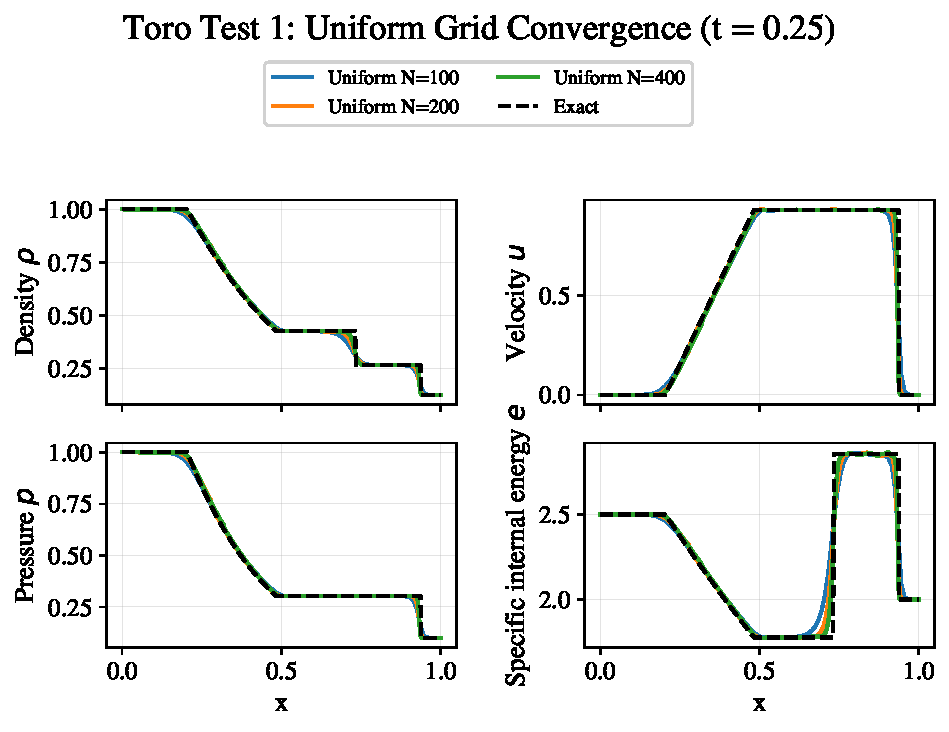
\includegraphics[width=\linewidth,trim=0 4 0 0,clip]
    {Fig02_fig_toro1d_test1_uniform.pdf}
    \caption{Toro Test 1 at $t_\mathrm{end}=0.25$: uniform-grid refinement sequence ($N=100,200,400$) with exact overlays.}
    \label{fig:uniform_t1}
\end{figure}

\begin{figure}[!tbp]
    \centering
    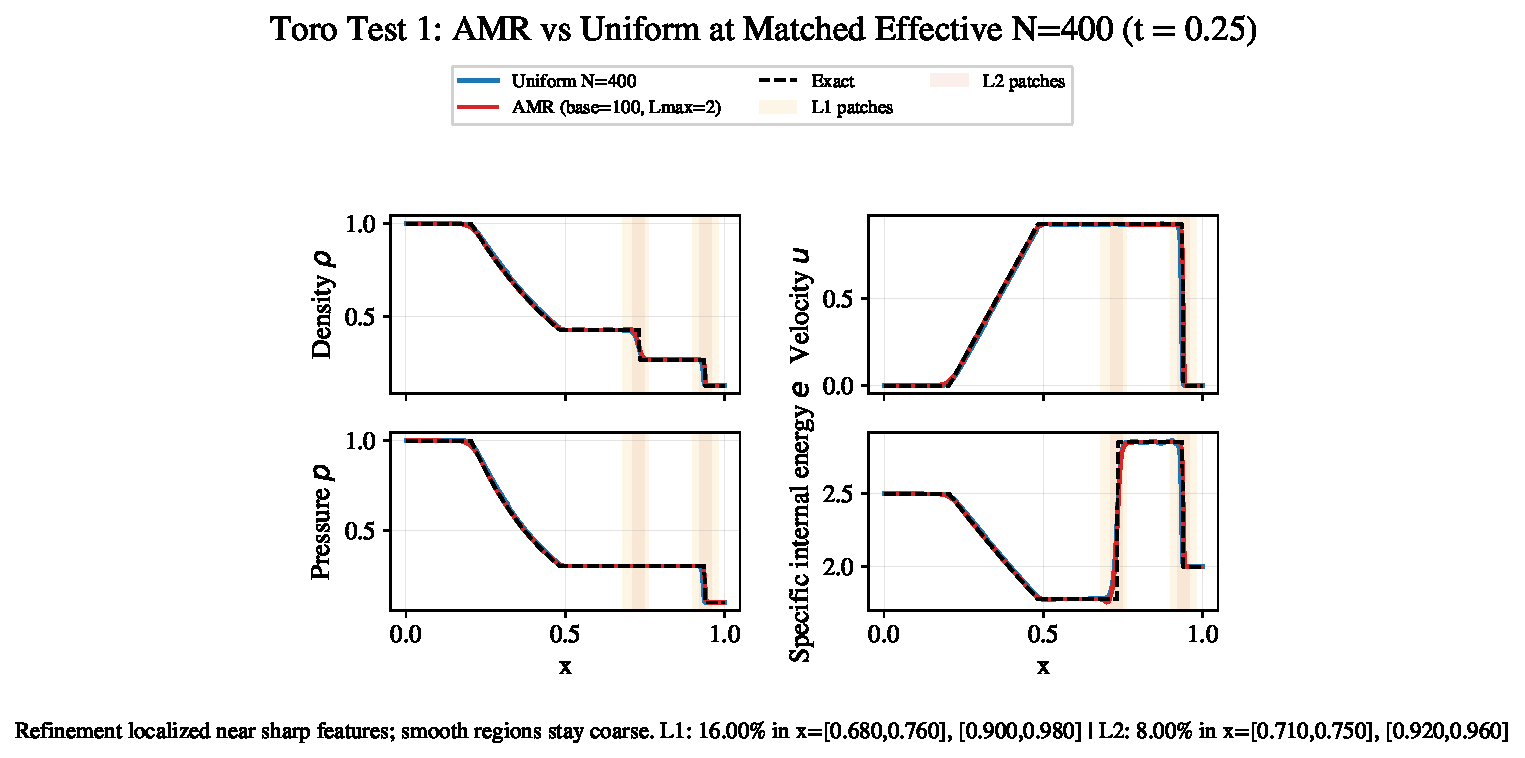
\includegraphics[width=\linewidth,trim=0 4 0 0,clip]{Fig03_fig_toro1d_test1_amr_vs_uniform.pdf}
    \caption{Toro Test 1 at $t_\mathrm{end}=0.25$: AMR versus uniform at matched $N_\mathrm{eff}=400$.}
    \label{fig:amr_vs_uniform_t1}
\end{figure}


AMR localisation is consistent with these profiles. At $N_\mathrm{eff}=400$, final refined coverage is 16\%/8\% (levels 1/2) for Test 1 and 48\%/44\% for Test 5, illustrating sparse versus broad refinement.

Updated-cell work-proxy ratios (AMR/uniform) are compared with runtime ratios, where the work proxy counts conserved-state updates only (Section~\ref{sec:methodology}). Mean updated-cell ratios are 1.000 ($N_\mathrm{eff}=100$), 0.730 ($N_\mathrm{eff}=200$), and 0.948 ($N_\mathrm{eff}=400$), while mean runtime ratios are 1.107, 1.297, and 1.370. In this short 1D workload, hierarchy overhead can dominate wall-clock time even when the update count drops. Task 1 therefore validates shock behaviour and matched-spacing accuracy, but not an AMR runtime advantage.

\begin{figure}[!tbp]
    \centering
    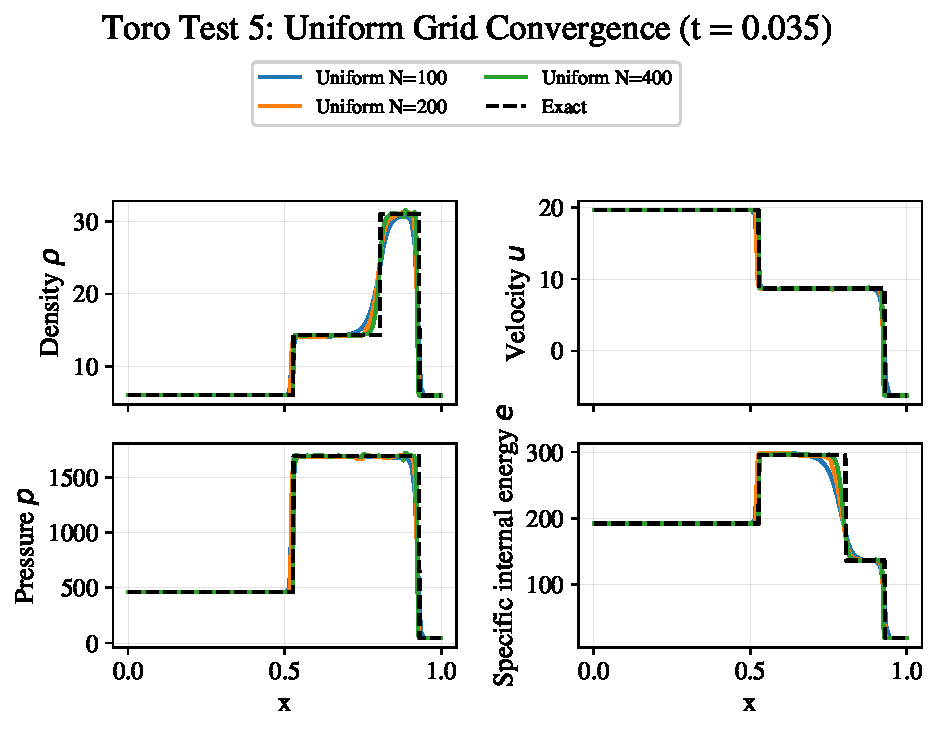
\includegraphics[width=\linewidth,trim=0 4 0 0,clip]{Fig04_fig_toro1d_test5_uniform.pdf}
    \caption{Toro Test 5 at $t_\mathrm{end}=0.035$: uniform-grid refinement sequence ($N=100,200,400$) with exact overlays.}
    \label{fig:uniform_t5}
\end{figure}

\begin{figure}[!tbp]
    \centering
    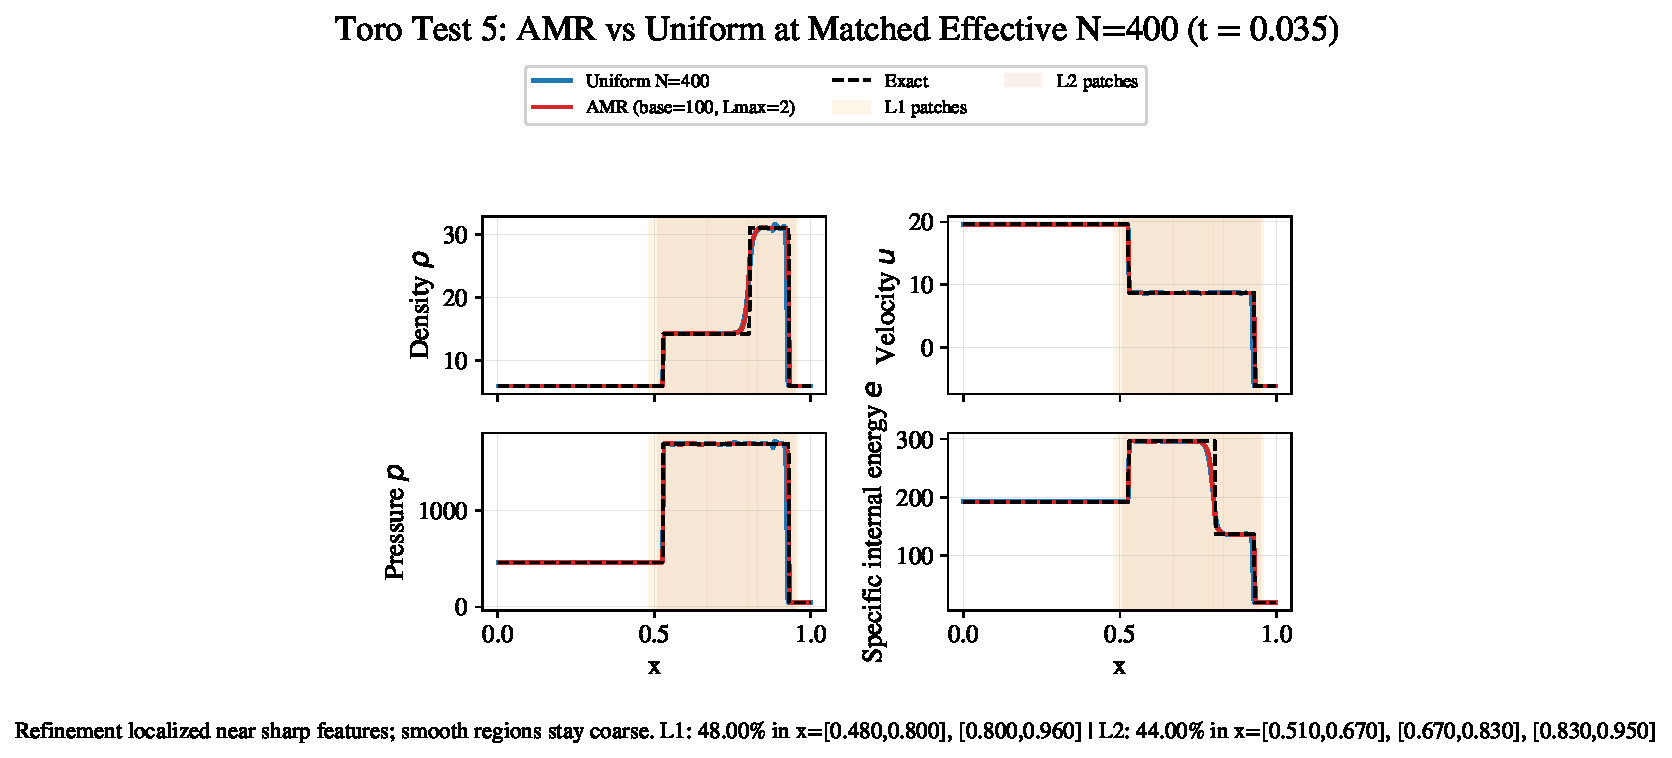
\includegraphics[width=\linewidth,trim=0 4 0 0,clip]{Fig05_fig_toro1d_test5_amr_vs_uniform.pdf}
    \caption{Toro Test 5 at $t_\mathrm{end}=0.035$: AMR versus uniform at matched $N_\mathrm{eff}=400$ with refinement bands.}
    \label{fig:amr_vs_uniform_t5}
\end{figure}

\subsection{Smooth-Flow Convergence}

Because the shock tubes cannot test smooth design order, a supplementary single-level case advects the Gaussian entropy perturbation from Section~\ref{sec:methodology} on uniform grids $N=\{128,256,512\}$ to $t_\mathrm{end}=0.05$. The reference solution is the same Gaussian shifted by $(u_0 t_\mathrm{end},v_0 t_\mathrm{end})$ and sampled on the same mesh. Density is retained as the scalar transport diagnostic.

Table~\ref{tab:smooth_convergence} shows $L_1(\rho)$ decreasing from $1.04\times10^{-5}$ to $3.01\times10^{-6}$ to $8.42\times10^{-7}$, with observed orders 1.79 and 1.84; the corresponding $L_2(\rho)$ orders are 1.62 and 1.63. This approaches the expected second-order trend in smooth transport.

A companion one-level AMR Gaussian test at effective $N_\mathrm{eff}=\{128,256,512\}$ does not recover the same trend: its density $L_1$ errors are $1.51\times10^{-5}$, $1.01\times10^{-5}$, and $7.58\times10^{-6}$, with observed orders 0.58 and 0.41. A stronger periodic two-level smooth-sinusoid check is also unfavourable: level-2 coverage is 100\% at all three effective resolutions, pressure-floor triggers remain zero, and the density $L_1$ orders are only 1.14 and 0.36. The missing multilevel smooth order therefore cannot be attributed simply to under-tagging or pressure-floor activation.\pathnote{new_campaign/Euler_AmrLevel/Exec/Euler1D/results_smooth_amr_convergence_20260308_001836/checks/smooth_amr_convergence.md} The conclusion from this subsection is asymmetric: the base discretisation shows the expected smooth single-level trend, but the present dataset does not justify the same claim for multilevel AMR.

\begin{table}[!htbp]
\centering
\scriptsize
\resizebox{\linewidth}{!}{%
\begin{tabular}{@{}c c c c c c@{}}
\hline
$N$ & $\Delta x$ & $L_1(\rho)$ & $p_{\mathrm{obs}}$ & $L_2(\rho)$ & $p_{\mathrm{obs}}$ \\
\hline
128 & $7.8125\times10^{-3}$ & $1.041\times10^{-5}$ & -- & $4.485\times10^{-5}$ & -- \\
256 & $3.90625\times10^{-3}$ & $3.014\times10^{-6}$ & 1.788 & $1.460\times10^{-5}$ & 1.619 \\
512 & $1.953125\times10^{-3}$ & $8.416\times10^{-7}$ & 1.841 & $4.719\times10^{-6}$ & 1.630 \\
\hline
\end{tabular}
}
\caption{Supplementary single-level smooth Gaussian entropy-perturbation test on uniform grids with $\rho=1+0.05\exp(-r^2/0.12^2)$, $(u,v,p)=(0.2,0.15,1.0)$, and $t_\mathrm{end}=0.05$.\pathnote{Euler_AmrLevel/Exec/Euler1D/results_smooth_entropy_convergence_20260306_044020/checks/smooth_entropy_convergence.csv; Euler_AmrLevel/Exec/Euler1D/results_smooth_entropy_convergence_20260306_044020/logs/smooth_num_n128.log}}
\label{tab:smooth_convergence}
\end{table}

\FloatBarrier

\subsection{Two-Dimensional Orientation Consistency}

Task 2 asks whether the two-dimensional implementation is orientation-consistent in the axis-aligned limit and how it behaves once the discontinuity is oblique. The Toro suite is therefore extended to two dimensions with $x$-split, $y$-split, and diagonal discontinuities. Uniform and AMR runs are again compared at matched finest spacing (uniform $400\times400$, AMR base $200\times200$ with one factor-2 refined level).

Axis-aligned rotational consistency is evaluated by comparing the $x$-split centreline at $y=0.5$ to the $y$-split centreline at $x=0.5$ after mapping the normal velocity component ($u\leftrightarrow v$). For uniform runs, the maximum reported rotation residual is $L_\infty=0$ over all tested variables and cases; AMR runs remain near machine precision, with maximum residual $L_\infty=1.55\times10^{-11}$. This holds for these effectively one-dimensional axis-aligned setups and is not a general claim of bitwise determinism for arbitrary 2D flows.

\begin{figure}[!htbp]
    \centering
    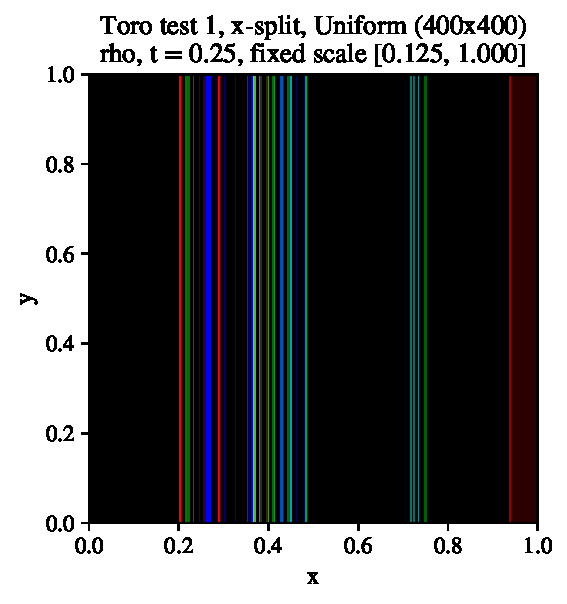
\includegraphics[width=0.95\linewidth,trim=0 4 0 0,clip]
    {Fig06_rho_t1_xsplit_uniform.pdf}
    \caption{Toro Test 1 ($x$-split): uniform $400\times400$ density at matched finest spacing, used as the axis-aligned reference orientation.}
    \label{fig:task2_xsplit_uniform}
\end{figure}


Table~\ref{tab:task2_rho} gives $x$-split centreline density errors against 1D exact references. The corresponding $y$-split errors are numerically identical to the reported precision in the compact metrics, so the axis-aligned 2D setups reproduce the 1D reference equally in both orientations. AMR improves or matches four of five tests.

\begin{table}[!htbp]
\centering
\small
\begin{tabular}{@{}c c c c@{}}
\hline
Test & Uniform $L_1(\rho)$ & AMR $L_1(\rho)$ & AMR/Uniform \\
\hline
1 & $5.134\times10^{-3}$ & $3.977\times10^{-3}$ & 0.775 \\
2 & $1.305\times10^{-2}$ & $8.367\times10^{-3}$ & 0.641 \\
3 & $6.107\times10^{-2}$ & $5.901\times10^{-2}$ & 0.966 \\
4 & $5.774\times10^{-2}$ & $5.885\times10^{-2}$ & 1.019 \\
5 & $3.660\times10^{-1}$ & $2.049\times10^{-1}$ & 0.560 \\
\hline
\end{tabular}
\caption{Two-dimensional $x$-split centreline density errors against 1D exact references.\pathnote{Task2/outputs/checks/task2_metrics_long.csv}}
\label{tab:task2_rho}
\end{table}

Variable-wise means for the $x$-split exact comparison are 0.792 ($\rho$), 0.764 ($u$), 0.671 ($p$), and 0.851 ($e_{\mathrm{int}}$), so the density table is representative rather than exceptional. Per-test geometric means over variables are 0.688, 0.692, 0.917, 1.025, and 0.435 for Tests 1--5, leaving Test 4 as the only slight aggregate preference for uniform.

\begin{figure}[!htbp]
    \centering
    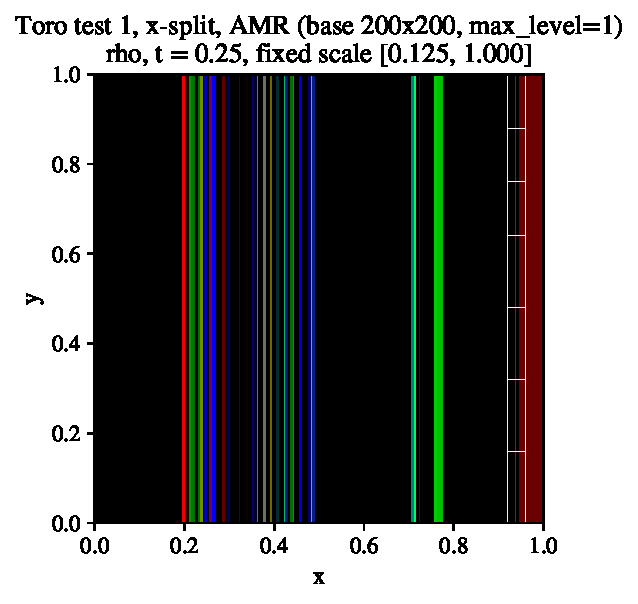
\includegraphics[width=0.95\linewidth,trim=0 4 0 0,clip]{Fig07_rho_t1_xsplit_amr_with_patches.pdf}
    \caption{Toro Test 1 ($x$-split): AMR density with patch overlay at $t_\mathrm{end}=0.25$, showing the essentially one-dimensional axis-aligned reference case.}
    \label{fig:task2_xsplit_amr}
\end{figure}


Diagonal splits form a stronger orientation stress test. A diagonal symmetry diagnostic compares $\rho(x,0.5)$ and $\rho(0.5,y)$ in the same run. AMR/uniform density-$L_1$ ratios are 1.271, 2.469, 4.225, 5.058, and 0.814 (Tests 1--5), identifying Tests 3 and 4 as the hardest diagonal cases.

Representative Test 4 provides suggestive, rather than conclusive, evidence for a patch-fragmentation mechanism. The diagonal AMR case refines a slightly larger area than the corresponding $x$-split case, but with much more fragmented level-1 patching: 25 boxes instead of 7.

\begin{table}[!htbp]
\centering
\small
\begin{tabular}{@{}l c c@{}}
\hline
Case & Level-1 boxes & Level-1 refined area \\
\hline
$x$-split AMR & 7 & 10.00\% \\
Diagonal AMR & 25 & 14.96\% \\
\hline
\end{tabular}
\caption{Representative Task 2 mechanism check for Toro Test 4. Level-1 box metadata are taken from the final AMR plotfiles; the corresponding AMR/uniform diagonal symmetry ratio is $5.058$.\pathnote{Euler_AmrLevel/Exec/Euler1D/results_task2_2d_fullmatrix_20260302_1957/checks/task2_diagonal_mechanism.csv; Task2/outputs/checks/task2_metrics_long.csv}}
\label{tab:task2_diag_mechanism}
\end{table}

Fragmented patching increases coarse--fine interface exposure and is consistent with the larger diagonal symmetry residual. Task 2 therefore supports strong axis-aligned consistency while identifying diagonal discontinuities as a materially harder AMR case rather than a generic solver failure. Figure~\ref{fig:task2_diag_amr} illustrates the harder diagonal Test~4 case.

\begin{figure}[!htbp]
  \centering
  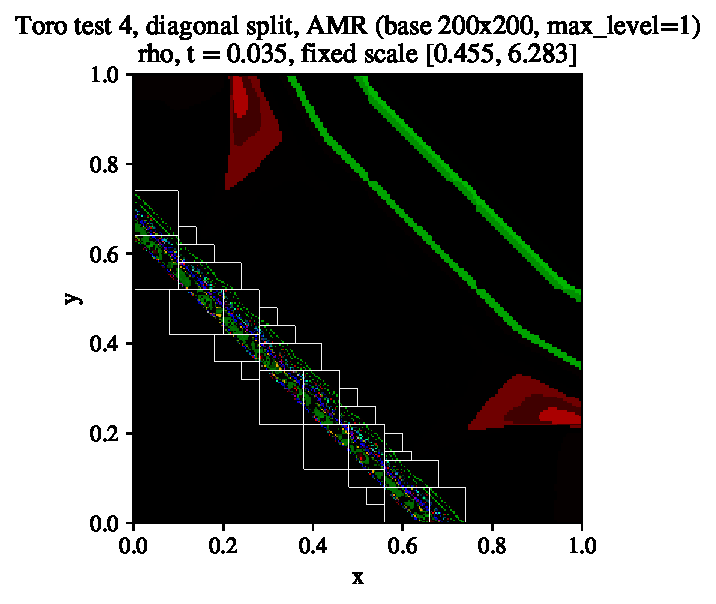
\includegraphics[width=0.95\linewidth,trim=0 4 0 0,clip]{Fig08_rho_t4_diag_amr_with_patches.pdf}
  \caption{Toro Test 4 (diagonal): matched-spacing AMR density with patch overlay at $t_\mathrm{end}=0.035$, illustrating the harder diagonal case discussed in Table~\ref{tab:task2_diag_mechanism}.}
  \label{fig:task2_diag_amr}
\end{figure}


\FloatBarrier

\subsection{Quadrant Timing, Scaling, and Sensitivity}

Task 3 asks whether the uniform benchmark exhibits the expected resolution-cost law, whether AMR reduces serial cost at matched finest spacing, and how much additional benefit survives under MPI on the same node. The quadrant benchmark uses the Lax-Liu initial data from Table~\ref{tab:quadrant_initial_data} with $t_\mathrm{end}=0.3$ \cite{lax1998}. Uniform one-rank timings scale nearly cubically: resolution-doubling runtime ratios are 8.23 (1536/768) and 8.07 (3072/1536), with effective exponents in $T\sim N^\alpha$ of 3.04 and 3.01.

At matched finest spacing, AMR cuts single-core runtime to $135.78\,\mathrm{s}$ at $N_\mathrm{eff}=1536$ (single run) and $315.04\pm0.31\,\mathrm{s}$ at $N_\mathrm{eff}=3072$ ($n=3$). These correspond to speedups of $4.32\times$ and $14.67\times$ relative to the uniform serial baselines, so the single-CPU comparison in part 3 is unambiguous.

Across all measured high-resolution AMR+MPI runs, the fastest single runtime is $137.45\,\mathrm{s}$ at $p=4$, corresponding to a $33.61\times$ speedup against the repeated uniform $N=3072$ serial baseline. The fastest repeated configuration is also $p=4$, with $138.63\pm1.03\,\mathrm{s}$ ($n=3$) and a combined speedup of $33.33\times$. This headline number matters only after decomposition, because otherwise an algorithmic gain can be mistaken for a parallel one.

Moving from uniform $N=3072$ serial to AMR serial reduces runtime by $4.31\times10^3\,\mathrm{s}$, while AMR $p=1\to4$ reduces a further 176\,s. Measured as a fraction of the absolute wall-clock reduction from uniform ($N=3072$) to the repeated $p=4$ configuration, AMR localisation accounts for $\approx 96.1\%$ of the reduction and MPI accounts for $\approx 3.9\%$ on this platform.

\begin{table}[!htbp]
\centering
\small
\begin{tabularx}{\linewidth}{@{}X r@{}}
\hline
Metric & Value \\
\hline
Uniform runtime, $N=3072$, $p=1$ ($n=3$) & $4.62\times10^{3}\pm5.53\times10^{1}\,\mathrm{s}$ \\
AMR runtime, effective $3072$, $p=1$ ($n=3$) & $315.04\pm0.31\,\mathrm{s}$ \\
AMR runtime, effective $3072$, $p=4$ ($n=3$) & $138.63\pm1.03\,\mathrm{s}$ \\
Algorithmic speedup (uniform $3072$ / AMR $p=1$) & $14.67\times$ \\
MPI speedup on AMR ($p=1$ to $p=4$) & $2.27\times$ \\
Combined speedup (uniform $3072$ / AMR $p=4$) & $33.33\times$ \\
\hline
\end{tabularx}
\caption{Performance decomposition at highest effective resolution using the repeated uniform serial baseline and repeated AMR serial/$p=4$ timings.\pathnote{Task3/outputs/report_pack_task3/task3_summary.md}}
\label{tab:timing_decomposition}
\end{table}

Strong-scaling gains flatten beyond about four ranks in the high-resolution AMR sweep: the repeated mean drops from $315.04\,\mathrm{s}$ at $p=1$ to $138.63\,\mathrm{s}$ at $p=4$, then changes only marginally to $140.40\,\mathrm{s}$ at $p=8$ before degrading to $166.57\,\mathrm{s}$ at $p=16$. The completed uniform $N=3072$ sweep shows the same qualitative ceiling, peaking at $3.16\times$ speedup for $p=8$ and slipping to $3.04\times$ at $p=16$, so the saturation pattern is not AMR-specific. Table~\ref{tab:efficiency_drop} reports efficiency $E(p)=T(1)/(pT(p))$ for representative uniform and AMR configurations.

Efficiency remains high at $p=2$ (0.866) but falls to 0.568 at $p=4$, 0.280 at $p=8$, and 0.118 at $p=16$ for the high-resolution AMR case. Instrumented diagnostic runs show the advance fraction falling from 65.9\% to 38.4\%, while FillPatch rises from 14.4\% to 24.2\% and reflux rises from 6.3\% to 15.2\%; tagging remains small at 2.1--3.1\%. This is consistent with higher relative costs from multilevel communication and synchronisation once per-rank update work becomes small.

The same instrumented runs report zero pressure-floor activations, and the reset also remains inactive in representative Task 1 Test 5 AMR and Task 2 diagonal Test 4 AMR cases. Within the runs examined here, the non-conservative energy reset is therefore a dormant safeguard rather than an active contributor to the reported solutions or timings.

\begin{table}[!htbp]
\centering
\small
\begin{tabular}{@{}c c c@{}}
\hline
Ranks & Uniform ($N=3072$) & AMR eff.\ ($N_\mathrm{eff}=3072$) \\
\hline
1 & 1.000 & 1.000 \\
2 & 0.900 & 0.866 \\
4 & 0.642 & 0.568 \\
8 & 0.395 & 0.280 \\
16 & 0.190 & 0.118 \\
\hline
\end{tabular}
\caption{Parallel efficiency decline with rank count in the completed uniform-$3072$ sweep and the matched AMR effective-$3072$ sweep.\pathnote{Task3/outputs/report_pack_task3/efficiency.csv}}
\label{tab:efficiency_drop}
\end{table}

A representative final-time density field for the effective-$3072$ AMR serial case is retained in Appendix~\ref{app:supplementary}. The finest patches track the curved shocks and contact structures that dominate the runtime and accuracy comparisons in this section. The uniform-resolution trend, matched-spacing serial comparison, and MPI saturation pattern are summarised in Figures~\ref{fig:time_vs_n}, \ref{fig:amr_vs_uniform_time}, and~\ref{fig:time_vs_cores}.

\begin{figure}[!tbp]
  \centering
  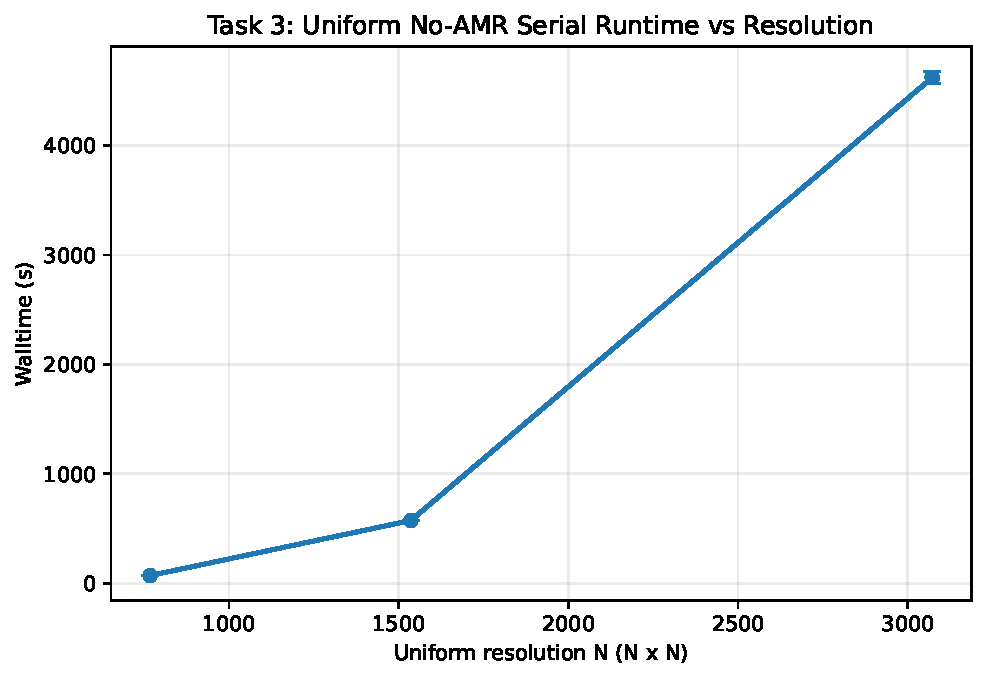
\includegraphics[width=\linewidth,trim=0 2 0 0,clip]{Fig09_time_vs_N.pdf}
  \caption{Uniform serial wall-clock runtime for the Task 3 quadrant problem at $t_\mathrm{end}=0.3$ as the grid is doubled from $768^2$ to $3072^2$, showing the near-cubic cost growth discussed in the text.}
  \label{fig:time_vs_n}
\end{figure}

\begin{figure}[!tbp]
  \centering
  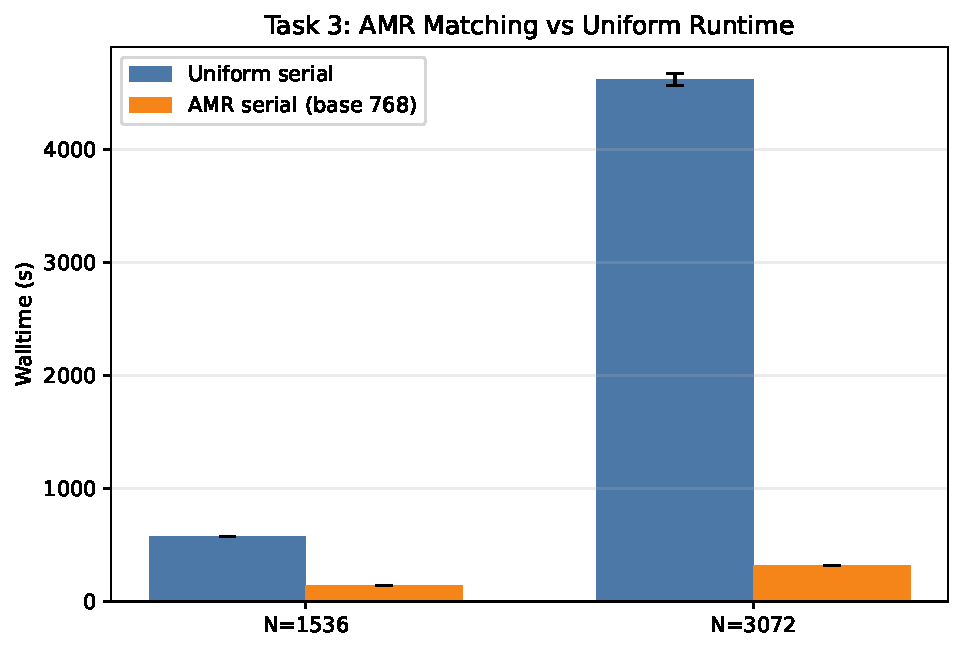
\includegraphics[width=\linewidth,trim=0 2 0 0,clip]{Fig10_AMR_vs_uniform_time.pdf}
  \caption{One-rank wall-clock runtime for uniform and AMR runs at matched effective resolutions $N_\mathrm{eff}=1536$ and $3072$, showing that most of the end-to-end gain arises before MPI is added.}
  \label{fig:amr_vs_uniform_time}
\end{figure}


\begin{figure}[!tbp]
  \centering
  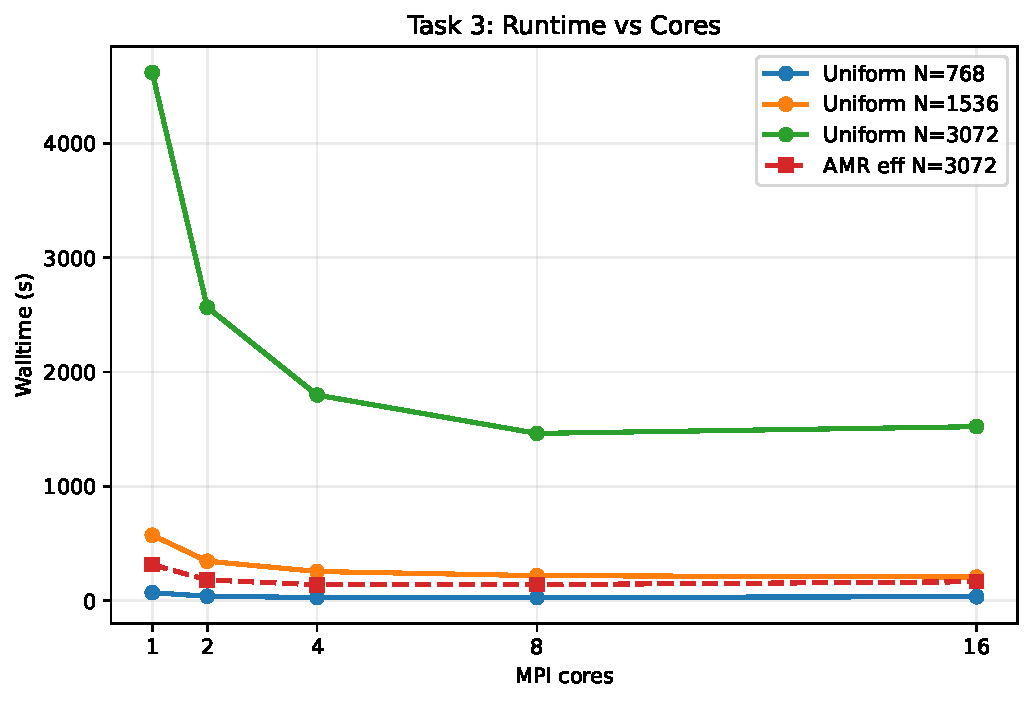
\includegraphics[width=\linewidth,trim=0 2 0 0,clip]{Fig11_time_vs_cores.pdf}
  \caption{Wall-clock runtime versus MPI rank count for the completed uniform $N=\{768,1536,3072\}$ sweeps and the AMR effective-$N_\mathrm{eff}=3072$ sweep on the same node. The main point is the same in both families: runtime improves up to a modest rank count and then saturates.}
  \label{fig:time_vs_cores}
\end{figure}


A separate one-at-a-time sensitivity study is performed around a one-level Task 3 baseline (\texttt{amr.blocking\_factor}=32, \texttt{amr.n\_error\_buf}=2, \texttt{tagging.phigrad}=0.1), rather than around the multi-level timing baseline used above. The biggest effect comes from \texttt{amr.blocking\_factor}: changing to 16 gives $-9.6\%$ runtime, while 64 gives $+18.1\%$. Increasing \texttt{amr.n\_error\_buf} from 2 to 4 gives $+8.0\%$, and decreasing to 1 gives $-1.1\%$. Threshold changes in \texttt{tagging.phigrad} are smaller (about $+3\%$). Baseline level-1 coverage is 7.81\%; it changes to 5.21\% (\texttt{blocking\_factor}=16) and 13.37\% (\texttt{blocking\_factor}=64), consistent with runtime direction. Patch geometry therefore matters more than modest threshold changes.

\begin{table}[!htbp]
\centering
\small
\begin{tabular}{@{}l c@{}}
\hline
Case & Runtime delta \\
\hline
\texttt{amr.blocking\_factor}=16 & $-9.6\%$ \\
\texttt{amr.blocking\_factor}=64 & $+18.1\%$ \\
\texttt{amr.n\_error\_buf}=1 & $-1.1\%$ \\
\texttt{amr.n\_error\_buf}=4 & $+8.0\%$ \\
\texttt{tagging.phigrad}=0.05 & $+3.0\%$ \\
\texttt{tagging.phigrad}=0.2 & $+3.5\%$ \\
\hline
\end{tabular}
\caption{One-at-a-time Task 3 runtime sensitivity relative to the separate one-level baseline defined in the text.\pathnote{Task3/outputs/report_pack_task3/sensitivity.csv; ANALYSIS_DERIVED_METRICS.md}}
\label{tab:sensitivity_delta}
\end{table}

A reproducibility check against a prior reference timing set finds a median absolute difference of 5.67\% over 29 matched configurations while preserving the same ordering and saturation trends.

A direct repeated uniform-$3072$ serial plotfile now supports both centreline and full-field checks against the same high-resolution baseline. In the full-field metric, uniform refinement from $N=768$ to $N=1536$ reduces $L_1(\rho)$ from $4.35\times10^{-3}$ to $2.15\times10^{-3}$, while AMR refinement from effective $N_\mathrm{eff}=1536$ to effective $N_\mathrm{eff}=3072$ reduces it from $6.13\times10^{-3}$ to $5.67\times10^{-3}$. At matched effective $N_\mathrm{eff}=1536$, the AMR/uniform full-field $L_1$ ratios are 2.852 for $\rho$, 2.323 for $u$, 2.320 for $v$, and 2.946 for $p$, so this stricter diagnostic does not support a blanket matched-spacing AMR accuracy advantage.\pathnote{new_campaign/Euler_AmrLevel/Exec/Euler1D/results_task3_accuracy_refresh_20260308_001536/checks/task3_fullfield_accuracy.md} Refinement still improves the quadrant solution in both families, but the Task 3 conclusion is deliberately split: the timing case for AMR is strong, whereas the matched-spacing accuracy case is improvement-with-refinement, not blanket superiority over uniform.

\FloatBarrier

\section{Discussion}
\label{sec:discussion}

\subsection{What Is Established About Accuracy}

The strongest accuracy claims are narrower than the raw number of tests might suggest, but they are well supported. The shock-dominated Toro suite shows the expected first-order-like global behaviour, and the supplementary smooth Gaussian test recovers near-second-order single-level convergence in density. Shock problems should not be read as formal design-order tests; the smooth single-level case is the cleaner probe of MUSCL+SSPRK2 away from discontinuities.

The same evidence also sets a clear boundary. The companion one-level AMR Gaussian test does not recover the uniform smooth trend, and a stronger periodic two-level smooth-sinusoid check remains low order even with full level-2 coverage and zero pressure-floor triggers. A multilevel smooth-convergence claim is therefore not supported.

At matched $N_\mathrm{eff}=400$, AMR is generally in the same accuracy class as uniform and often better in density and pressure, but it does not improve every case. Test 4 remains near-neutral or slightly worse in several aggregate measures. The cautious interpretation is therefore that AMR can preserve, and often modestly improve, shock-oriented accuracy at matched finest spacing without guaranteeing a smaller global norm for every morphology.

The two-dimensional orientation diagnostics support the same measured tone. Under the chosen centreline metric, uniform rotation residuals are exactly zero, while AMR residuals remain at $O(10^{-11})$. This is more naturally interpreted as a small multilevel-operation effect than as directional bias in the core flux implementation, although the present diagnostics do not prove that distinction.

For the diagonal difficulty, the representative Test 4 box metadata suggest a plausible mechanism rather than a proof. The diagonal AMR run uses 25 level-1 boxes over 14.96\% of the domain, whereas the $x$-split counterpart uses 7 boxes over 10.00\%. That pattern is consistent with extra coarse-fine interface exposure in the oblique case and therefore with larger diagonal symmetry residuals.

\subsection{Why AMR Does Not Guarantee Smaller Global Error}

Coverage, error, and runtime results highlight a central AMR tradeoff. When refinement remains localised and well aligned with the dominant structures, AMR concentrates resolution effectively. When refined coverage broadens or fragments, hierarchy-management costs rise and the AMR solution can move toward a near-uniform fine-grid regime without inheriting every advantage of that regime in global norms. The updated-cell work-proxy analysis makes this concrete: the proxy counts only conserved-state updates, whereas runtime and global error also reflect ghost fills, reflux, regridding, and coarse-fine interactions. Localisation is the mechanism behind the speedups in this report, but it is not a blanket guarantee of superior global accuracy.

\subsection{Where the Task 3 Speedup Comes From}

The key performance result is the decomposition at effective $N_\mathrm{eff}=3072$:
\begin{equation}
\label{eq:task3_speedup_decomposition}
\begin{aligned}
S_{\mathrm{total}}
&= \frac{T^{\mathrm{U}}_{3072,1}}{T^{\mathrm{A}}_{3072,4}}
= S_{\mathrm{alg}}\,S_{\mathrm{mpi}}, \\
S_{\mathrm{alg}}
&= \frac{T^{\mathrm{U}}_{3072,1}}{T^{\mathrm{A}}_{3072,1}}, \\
S_{\mathrm{mpi}}
&= \frac{T^{\mathrm{A}}_{3072,1}}{T^{\mathrm{A}}_{3072,4}}.
\end{aligned}
\end{equation}
Here, $\mathrm{U}$ and $\mathrm{A}$ denote run types; $S_{\mathrm{alg}}=14.67$, $S_{\mathrm{mpi}}=2.27$, and so $S_{\mathrm{total}}=33.33$.

This decomposition is the main interpretive step for Task 3 because the headline $33.33\times$ could otherwise be misread as a parallel result. It is not: most of the gain comes from AMR localisation at one rank, and MPI adds a smaller extra factor up to about four ranks, after which gains flatten and efficiencies fall sharply. The instrumented breakdown supports this reading directly: as rank count increases, the advance share drops while FillPatch and reflux account for a larger fraction of wall-clock time. This is consistent with standard strong-scaling limits \cite{amdahl1967}.

Measured by absolute runtime reduction, localisation accounts for about 96\% of the gain before MPI beyond one rank is added. MPI still improves best time-to-solution, but only as a secondary factor in this configuration. The related saturation pattern in the completed uniform-$3072$ sweep shows that the ceiling is not AMR-specific. For the assignment brief, the defensible statement is therefore that AMR is the dominant source of speedup here, while MPI provides a modest additional benefit before saturation.

\subsection{Claim Strength and Reproducibility}

The extra repeat work strengthens the timing argument because it tests ordering, not just isolated best runs. The pack-only rerun reproduces the ordering against the earlier reference set (median absolute difference 5.67\% over 29 matched configurations), and the refreshed repeated uniform sweeps remove the earlier repeat-depth asymmetry between the high- and lower-resolution uniform MPI timings. On the accuracy side, the direct repeated uniform-$3072$ reference sharpens the claim: both centreline and full-field diagnostics show improvement with refinement in the uniform and AMR families, but the full-field metric is less favourable to AMR at matched effective resolution. That counterexample should constrain the wording of the final claim.

\subsection{What Remains Unresolved}

The principal unresolved issue is the missing multilevel smooth-order recovery. Single-level smooth-flow convergence is demonstrated, but the companion one-level AMR smooth test does not recover the same order, and the stronger periodic two-level smooth-sinusoid check remains low order despite full level-2 coverage. The same periodic multilevel run nevertheless preserves the global conserved quantities extremely well: relative drifts are about $10^{-9}$ in mass and momentum and about $10^{-11}$ in total energy, so the missing smooth order is not explained by obvious loss of conservation in that representative case.\pathnote{new_campaign/Euler_AmrLevel/Exec/Euler1D/results_smooth_amr_convergence_20260308_001836/checks/smooth_conservation.md}

The quadrant accuracy trend is supported by centreline and full-field comparisons against one repeated uniform-$3072$ serial reference, but not by an exact solution. The profiling evidence is also informative but still coarse: a breakdown is available for FillPatch, advance, reflux, and tagging in representative Task 3 runs, yet MPI communication and regridding are not separated. Finally, all timing results are single-node and should not be generalised across architectures without additional runs.

Within these limits, the report supports three defensible conclusions: the solver passes the core shock-oriented checks, axis-aligned orientation behaviour is consistent, and AMR provides substantial end-to-end acceleration at matched finest spacing on the tested node.

\section{Conclusions}
\label{sec:conclusions}

\paragraph{Established.}
Three conclusions are supported directly by the reported evidence. First, the base solver shows the expected first-order-like global behaviour on shock-dominated Toro problems, while a supplementary smooth uniform advection test recovers near-second-order density convergence. Second, the two-dimensional implementation is directionally consistent for axis-aligned splits under the chosen diagnostics, whereas diagonal discontinuities are materially harder for the AMR hierarchy. Third, for the Task 3 quadrant benchmark on one node, AMR materially reduces time-to-solution at matched finest spacing, and the best repeated high-resolution configuration is the AMR $p=4$ case with a $33.33\times$ speedup over the repeated uniform $N=3072$ serial baseline.

\paragraph{What the assignment brief is answered by.}
These results answer the brief most clearly when the Task 3 speedup is decomposed rather than quoted in isolation. At effective $N_\mathrm{eff}=3072$, $14.67\times$ of the gain comes from AMR localisation at one rank and $2.27\times$ from MPI on the AMR case. The main performance result is therefore that AMR removes most of the unnecessary fine-grid work before MPI is added. On the accuracy side, the repeated uniform-$3072$ reference shows that refinement improves the quadrant solution in both the uniform and AMR families, but the stricter full-field diagnostic does not support a general matched-spacing AMR accuracy advantage.

\paragraph{Suggestive.}
Two interpretations are plausible and useful, but should remain qualified. The diagonal Test 4 metadata suggest that fragmented oblique patching amplifies coarse-fine interaction and therefore symmetry error. The Task 3 timing breakdown likewise suggests that FillPatch and reflux become increasingly important as rank count rises and per-rank update work falls. Both fit the observed data, but neither is established as a unique causal explanation.

\paragraph{Unresolved.}
The highest-priority unresolved issue is the missing multilevel smooth-order recovery. The present checks rule out simple explanations such as obvious under-tagging, pressure-floor activity, or gross loss of global conservation in a representative periodic case, but they do not identify the dominant multilevel error source. Next steps should prioritise a cleaner multilevel smooth-validation study, finer-grained profiling of AMR overheads and communication, and broader orientation tests beyond Riemann-style discontinuities.


\FloatBarrier
\appendix
\raggedbottom
\setcounter{table}{0}
\renewcommand{\thetable}{A.\arabic{table}}
\setcounter{figure}{0}
\renewcommand{\thefigure}{A.\arabic{figure}}


\section{Supplementary Plots}
\label{app:supplementary}
\subsection{Supplementary One-Dimensional Plots}

Additional one-dimensional Toro examples (uniform and AMR at matched finest spacing) are provided here to show both favourable and near-neutral AMR cases. All panels use the same plotting pipeline as the main figures, with exact references overlaid where available.

\begin{figure}[H]
\centering
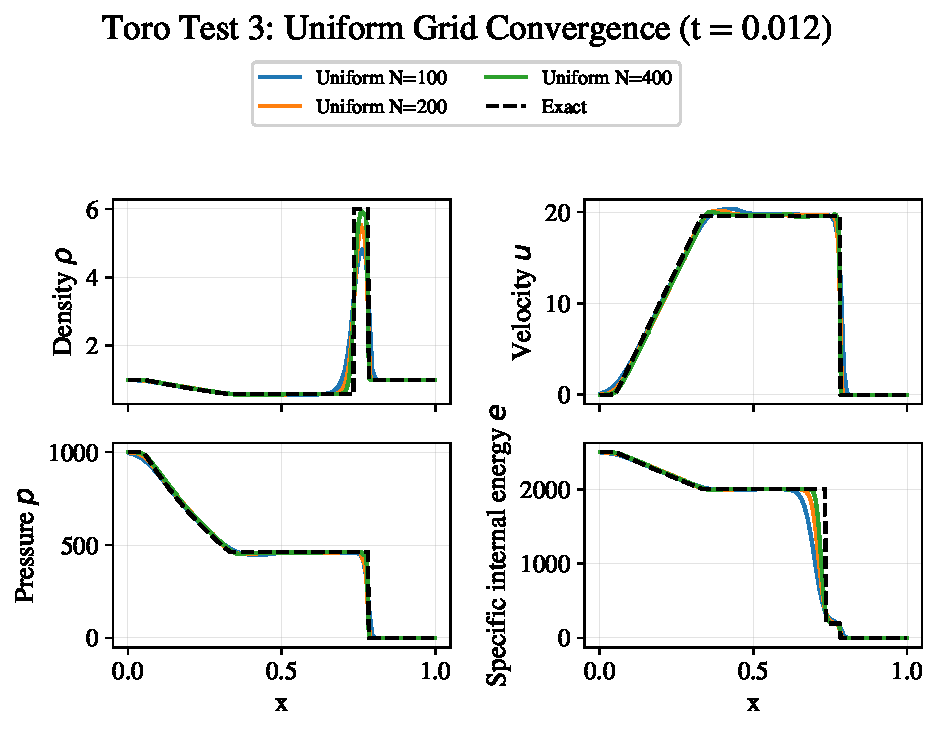
\includegraphics[width=\linewidth,trim=0 4 0 0,clip]{FigA1_fig_toro1d_test3_uniform.pdf}
\caption{Toro Test 3: uniform solutions at $N=\{100,200,400\}$ at $t_\mathrm{end}=0.012$, overlaid with the exact Riemann solution.}
\label{fig:app_t1_t3_uniform}
\end{figure}


\begin{figure}[H]
\centering
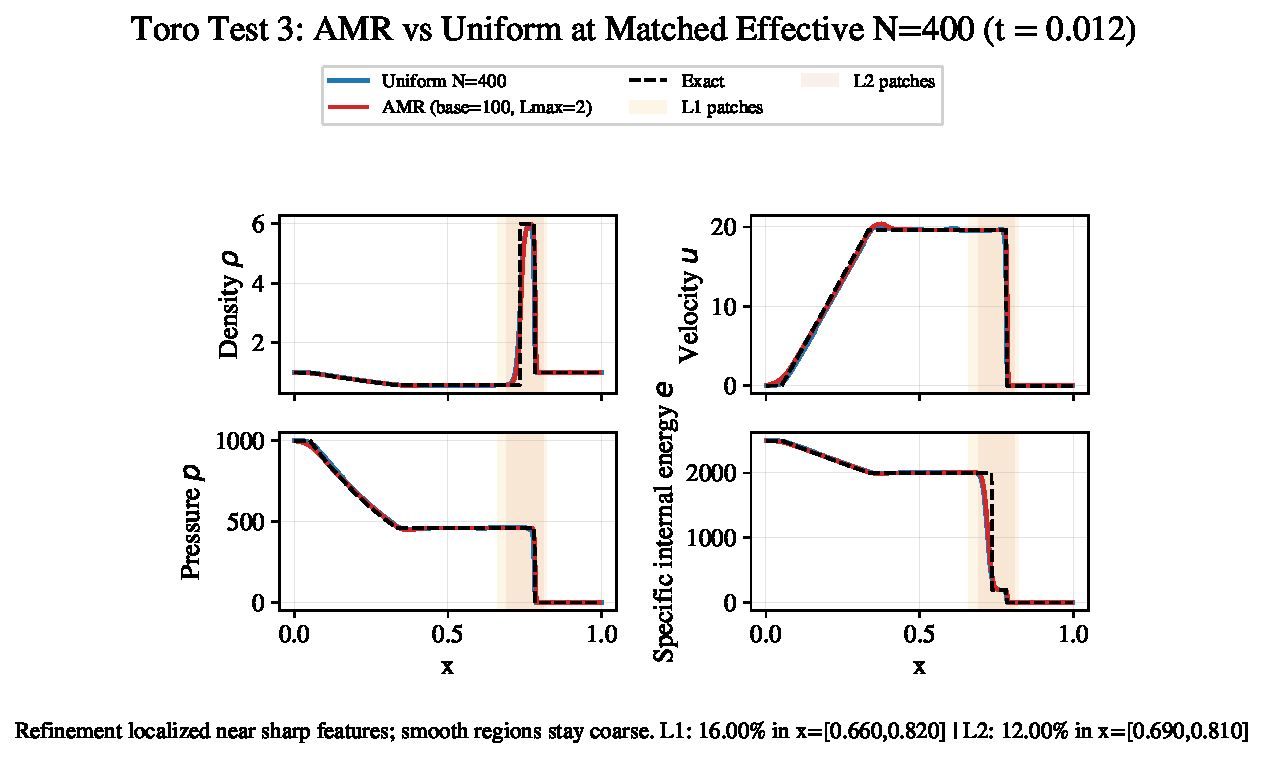
\includegraphics[width=\linewidth,trim=0 4 0 0,clip]{FigA2_fig_toro1d_test3_amr_vs_uniform.pdf}
\caption{Toro Test 3: AMR versus uniform at matched effective resolution ($N_{\mathrm{eff}}=400$), with refinement-band overlays.}
\label{fig:app_t1_t3_amr}
\end{figure}

\begin{figure}[H]
\centering
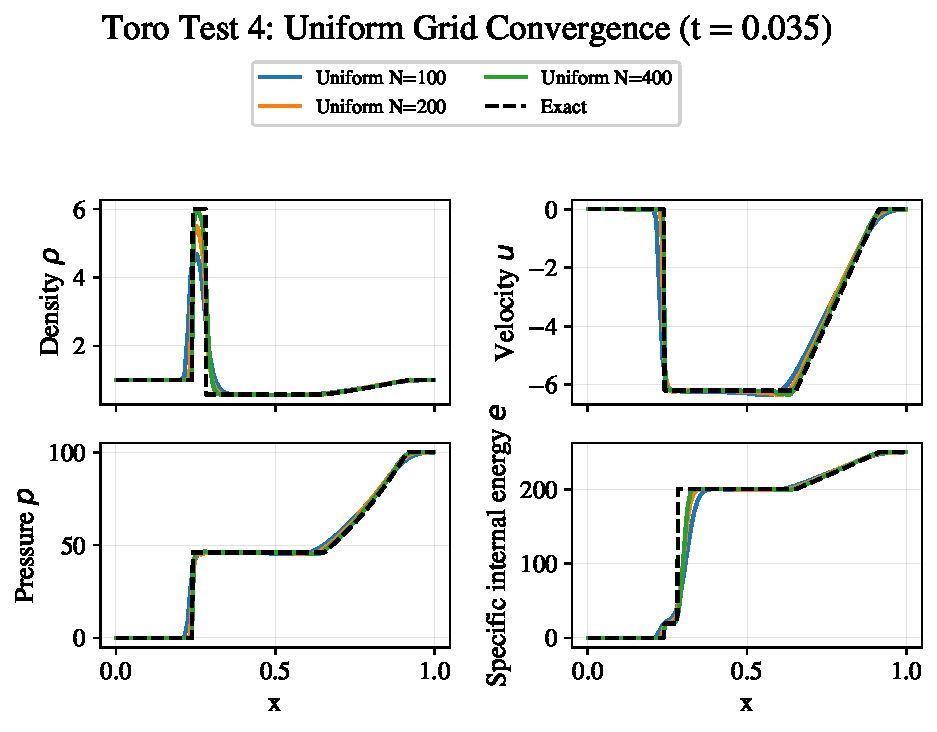
\includegraphics[width=\linewidth,trim=0 4 0 0,clip]{FigA3_fig_toro1d_test4_uniform.pdf}
\caption{Toro Test 4: uniform solutions at $N=\{100,200,400\}$ at $t_\mathrm{end}=0.035$, overlaid with the exact Riemann solution.}
\label{fig:app_t1_t4_uniform}
\end{figure}

\begin{figure}[H]
\centering
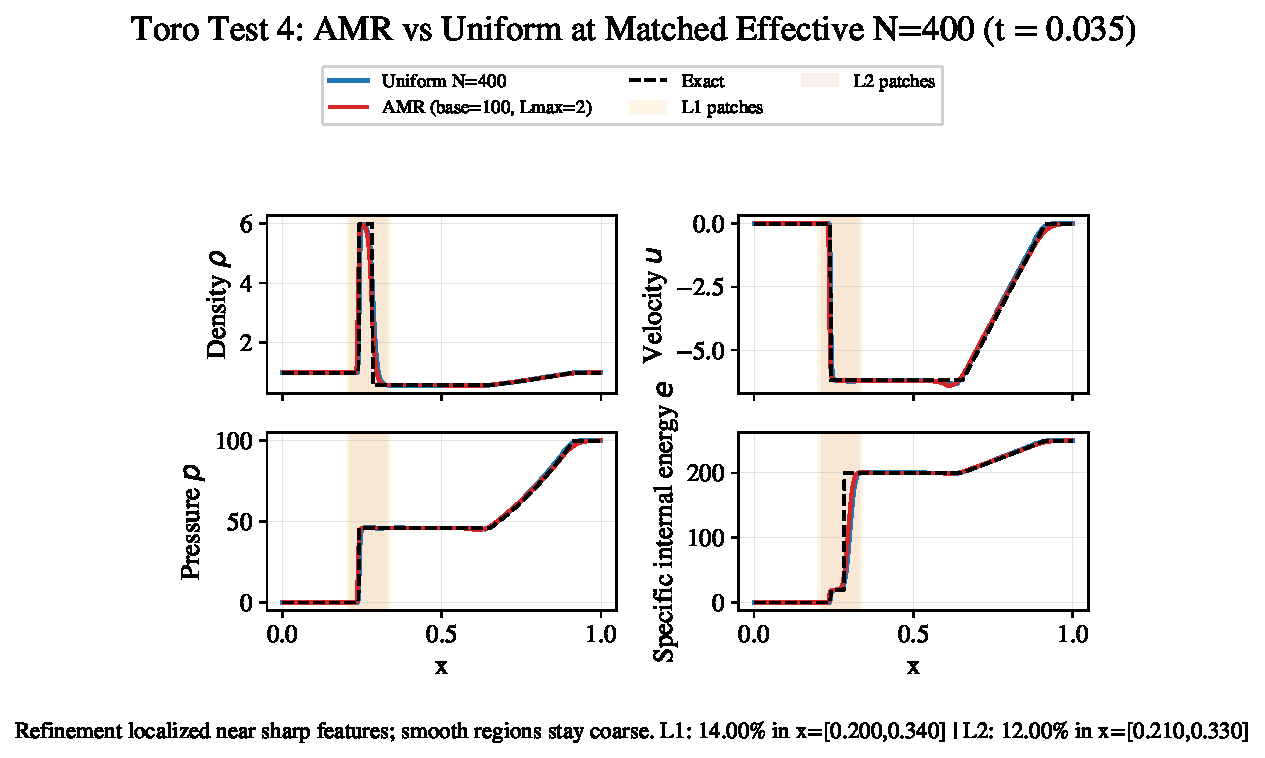
\includegraphics[width=\linewidth,trim=0 4 0 0,clip]{FigA4_fig_toro1d_test4_amr_vs_uniform.pdf}
\caption{Toro Test 4: AMR versus uniform at matched effective resolution ($N_{\mathrm{eff}}=400$), with refinement-band overlays.}
\label{fig:app_t1_t4_amr}
\end{figure}

\clearpage
\subsection{Supplementary Two-Dimensional Orientation Gallery}

Additional two-dimensional density snapshots $\rho(x,y)$ on $[0,1]\times[0,1]$ with AMR patch overlays are provided here as visual support for the orientation diagnostics in Section~\ref{sec:results}. Quantitative statements in the main text remain grounded in the tabulated norm outputs.

\begin{figure}[H]
\centering
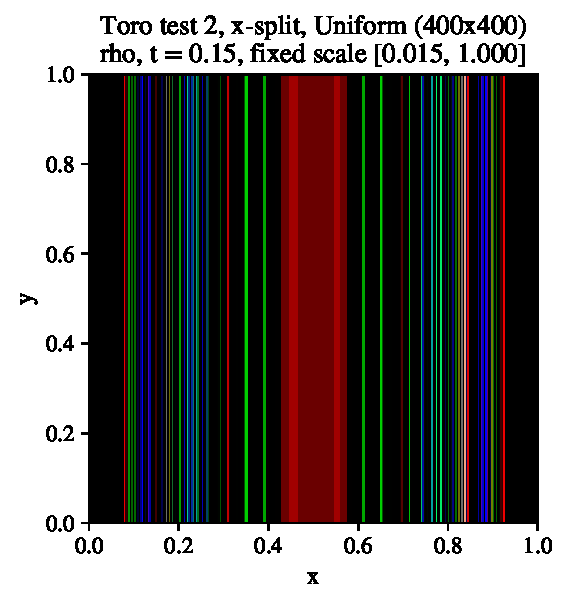
\includegraphics[width=\linewidth,trim=0 4 0 0,clip]{FigA5_rho_t2_xsplit_uniform.pdf}
\caption{Toro Test 2 ($t_\mathrm{end}=0.15$): $x$-split uniform density at $400\times 400$.}
\label{fig:app_t2_xsplit_uniform}
\end{figure}

\begin{figure}[H]
\centering
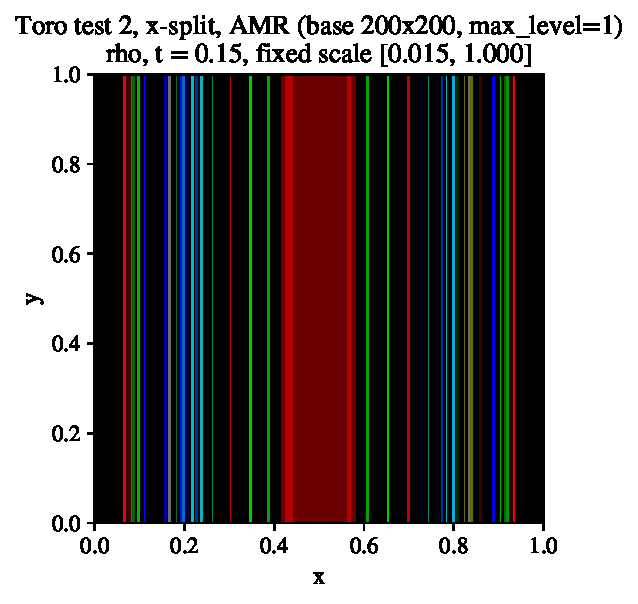
\includegraphics[width=\linewidth,trim=0 4 0 0,clip]{FigA6_rho_t2_xsplit_amr_with_patches.pdf}
\caption{Toro Test 2 ($t_\mathrm{end}=0.15$): $x$-split matched-spacing AMR density with patch overlay (effective $400\times 400$).}
\label{fig:app_t2_xsplit_amr}
\end{figure}

\begin{figure}[H]
\centering
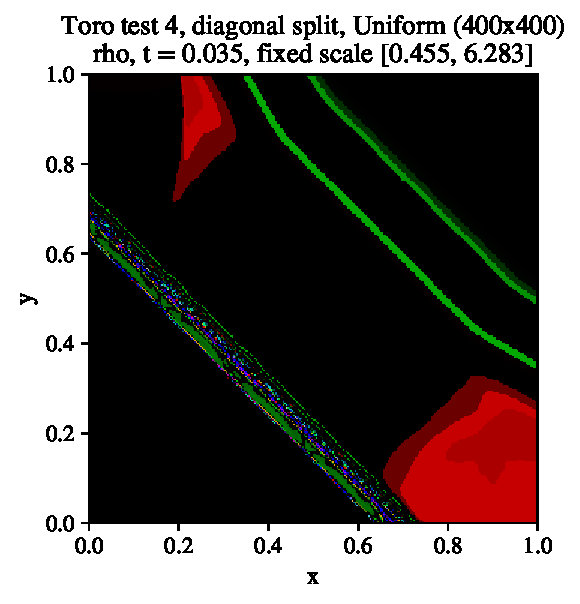
\includegraphics[width=\linewidth,trim=0 4 0 0,clip]{FigA7_rho_t4_diag_uniform.pdf}
\caption{Toro Test 4 ($t_\mathrm{end}=0.035$): diagonal discontinuity, uniform density at $400\times 400$.}
\label{fig:app_t4_diag_uniform}
\end{figure}

\begin{figure}[H]
\centering
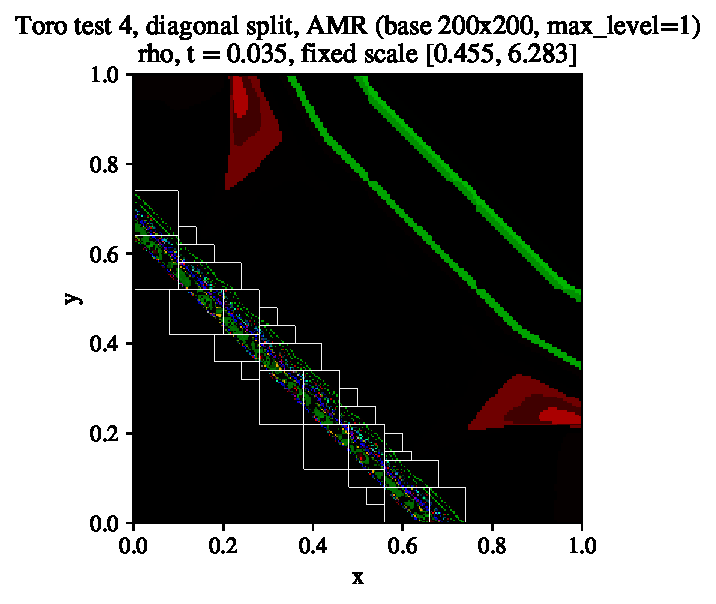
\includegraphics[width=\linewidth,trim=0 4 0 0,clip]{FigA8_rho_t4_diag_amr_with_patches.pdf}
\caption{Toro Test 4 ($t_\mathrm{end}=0.035$): diagonal discontinuity, matched-spacing AMR density with patch overlay.}
\label{fig:app_t4_diag_amr}
\end{figure}

\begin{figure}[H]
\centering
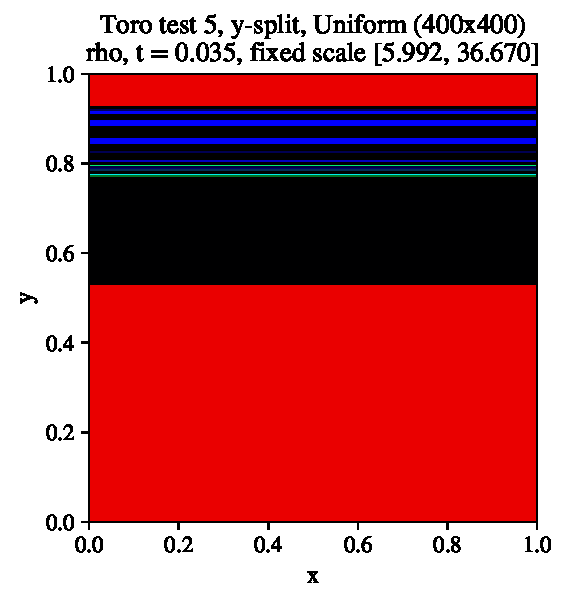
\includegraphics[width=\linewidth,trim=0 4 0 0,clip]{FigA9_rho_t5_ysplit_uniform.pdf}
\caption{Toro Test 5 ($t_\mathrm{end}=0.035$): $y$-split uniform density at $400\times 400$ (strong case).}
\label{fig:app_t5_ysplit_uniform}
\end{figure}

\begin{figure}[H]
\centering
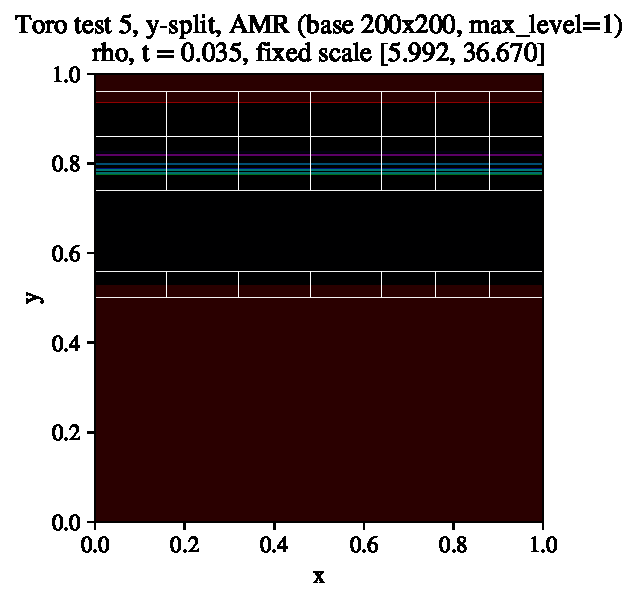
\includegraphics[width=\linewidth,trim=0 4 0 0,clip]{FigA10_rho_t5_ysplit_amr_with_patches.pdf}
\caption{Toro Test 5 ($t_\mathrm{end}=0.035$): $y$-split matched-spacing AMR density with patch overlay.}
\label{fig:app_t5_ysplit_amr}
\end{figure}

\clearpage
\subsection*{Supplementary Task 3 Timing Plots}

Additional Task 3 plots are retained here as supporting material for the main discussion.

\begin{figure}[H]
\centering
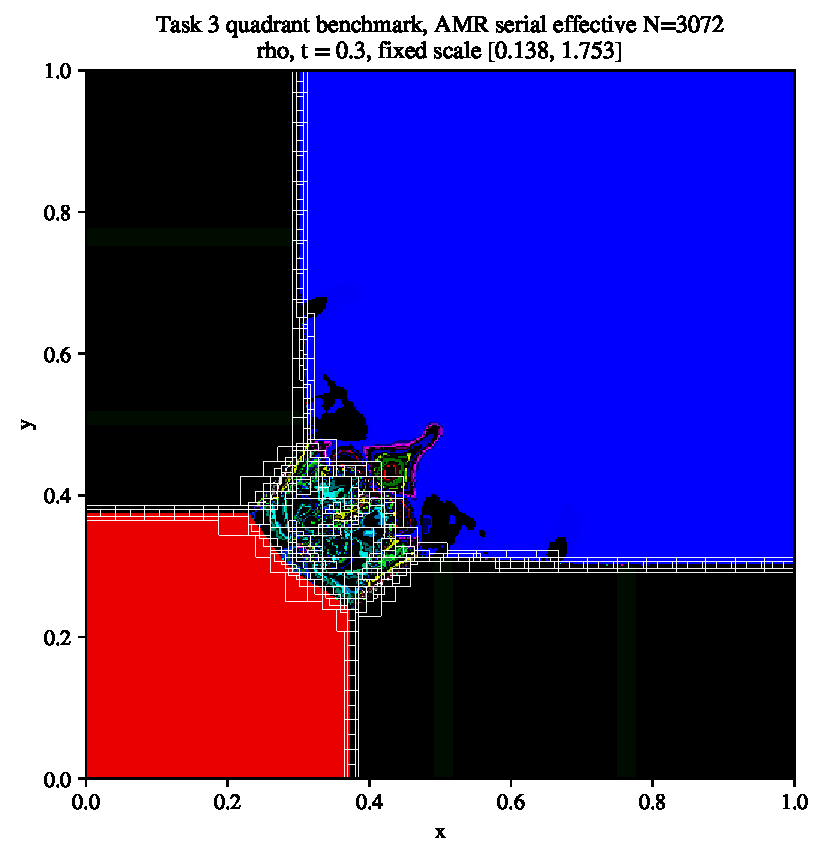
\includegraphics[width=0.92\linewidth,height=0.24\textheight,keepaspectratio]{FigA11_quadrant_rho_amr_eff3072.pdf}
\caption{Task 3 quadrant benchmark at $t_\mathrm{end}=0.3$: AMR density for base $768\times768$, \texttt{amr.max\_level=2} (effective $N_\mathrm{eff}=3072$), with final-time patch overlays showing localisation around the strongest curved features.}
\label{fig:task3_quadrant_amr}
\end{figure}

\begin{figure}[H]
\centering
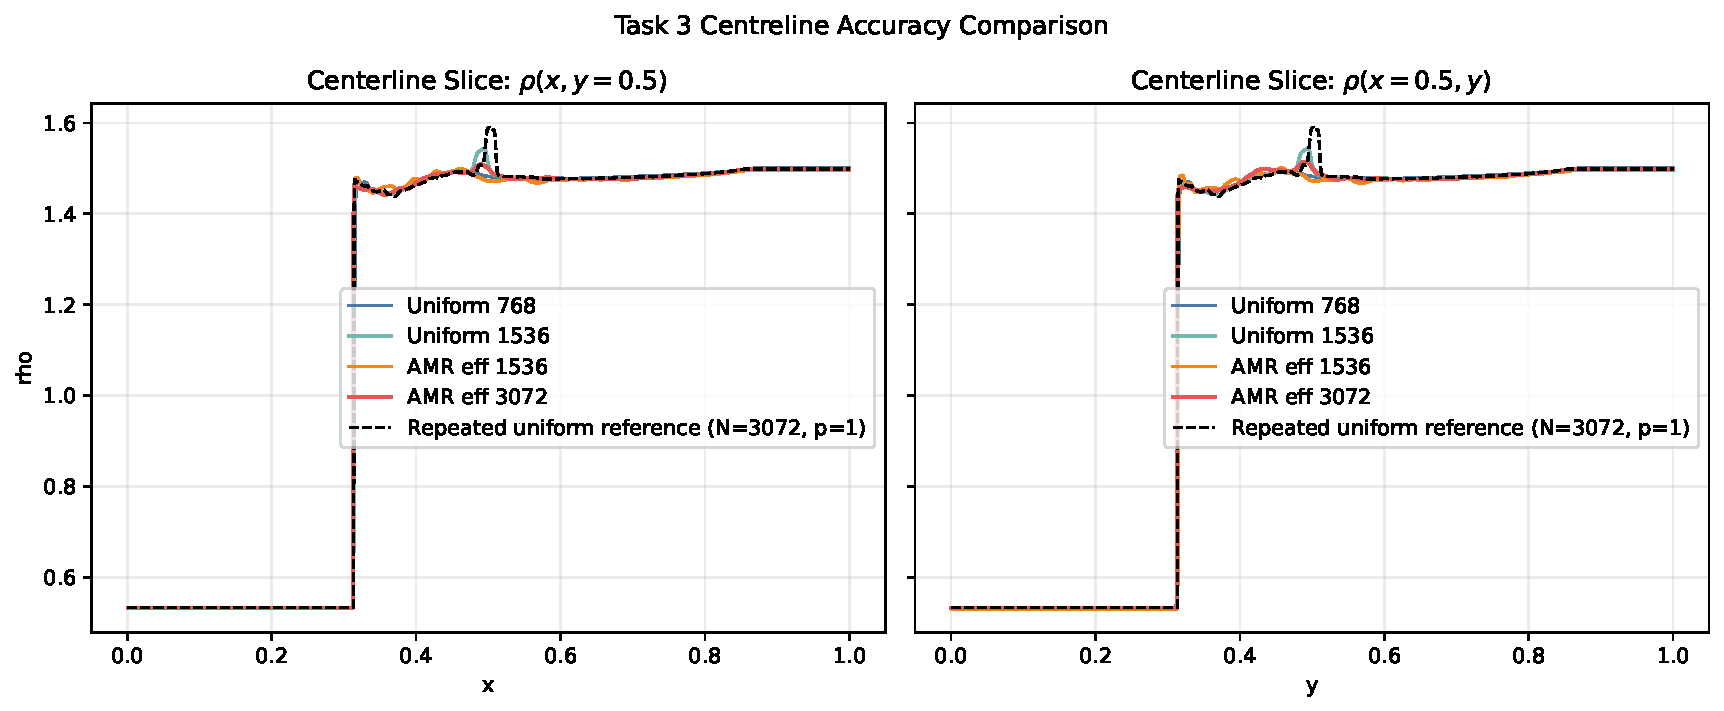
\includegraphics[width=0.92\linewidth,height=0.24\textheight,keepaspectratio,trim=0 4 0 0,clip]{FigA12_accuracy_slice_rho.pdf}
\caption{Centreline density comparison for the Task 3 direct-reference check at $t_\mathrm{end}=0.3$. Uniform $N=\{768,1536\}$ and AMR effective $N=\{1536,3072\}$ are compared against a repeated uniform $N=3072$ serial reference.}
\label{fig:accuracy_slice_rho}
\end{figure}

\begin{figure}[H]
\centering
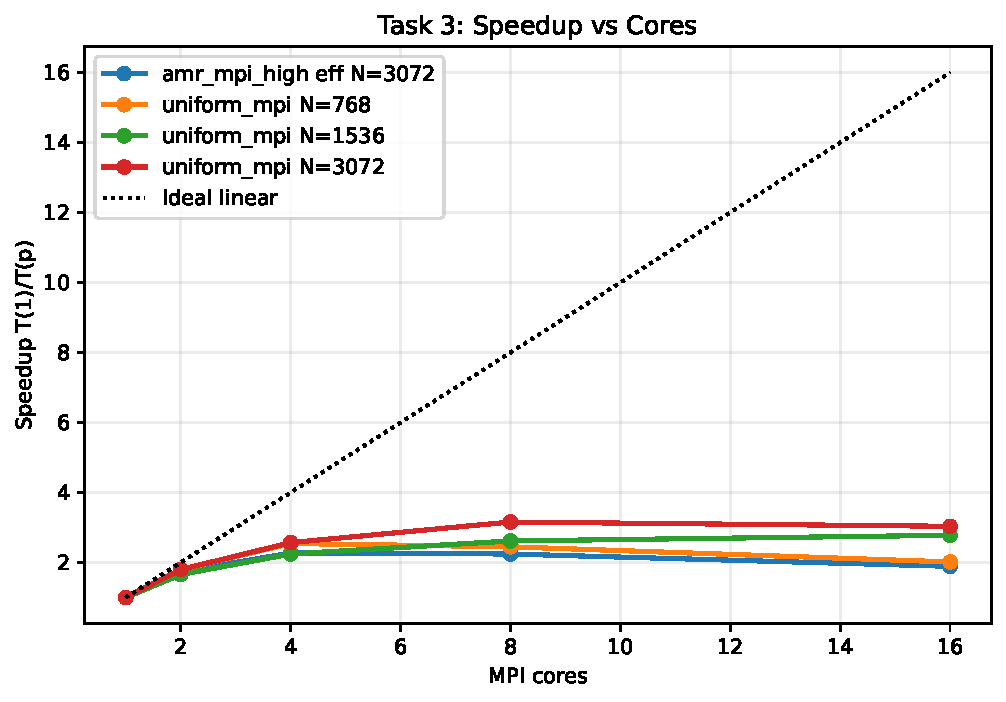
\includegraphics[width=0.92\linewidth,height=0.24\textheight,keepaspectratio,trim=0 4 0 0,clip]{FigA13_speedup_vs_cores.pdf}
\caption{Task 3 strong-scaling speedup $S(p)=T(1)/T(p)$ versus MPI rank count for the completed uniform $N=3072$ sweep and the AMR effective-$N_\mathrm{eff}=3072$ sweep.}
\label{fig:app_task3_speedup_vs_cores}
\end{figure}

\begin{figure}[H]
\centering
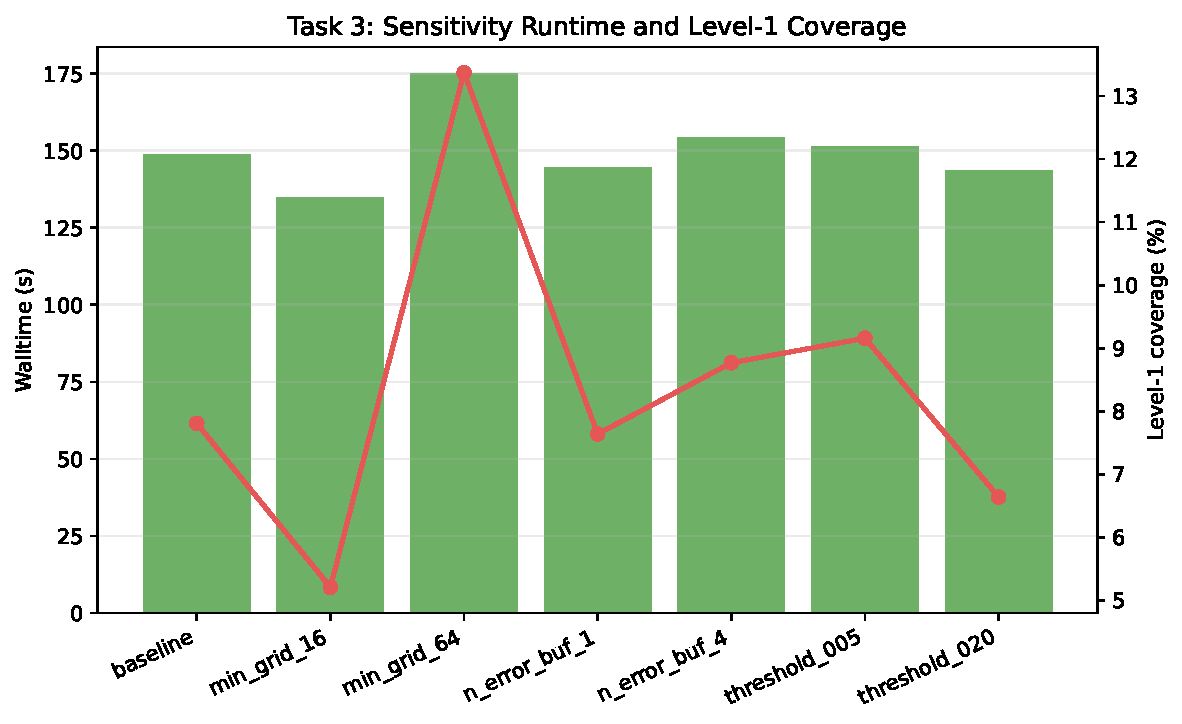
\includegraphics[width=0.92\linewidth,height=0.24\textheight,keepaspectratio,trim=0 4 0 0,clip]{FigA14_sensitivity_summary.pdf}
\caption{Task 3 runtime sensitivity of the separate one-level baseline to changes in the main AMR control parameters.}
\label{fig:app_task3_sensitivity_summary}
\end{figure}

\FloatBarrier


\begin{thebibliography}{1}
\expandafter\ifx\csname url\endcsname\relax
  \def\url#1{\texttt{#1}}\fi
\expandafter\ifx\csname urlprefix\endcsname\relax\def\urlprefix{URL }\fi
\expandafter\ifx\csname href\endcsname\relax
  \def\href#1#2{#2} \def\path#1{#1}\fi

\bibitem{toro2009}
E.~F. Toro, Riemann Solvers and Numerical Methods for Fluid Dynamics: A
  Practical Introduction, 3rd Edition, Springer, 2009.

\bibitem{berger1989}
M.~J. Berger, P.~Colella, Local adaptive mesh refinement for shock
  hydrodynamics, Journal of Computational Physics 82~(1) (1989) 64--84.
\newblock \href {https://doi.org/10.1016/0021-9991(89)90035-1}
  {\path{doi:10.1016/0021-9991(89)90035-1}}.

\bibitem{AMReX_JOSS}
W.~Zhang, A.~Almgren, V.~Beckner, J.~Bell, J.~Blaschke, C.~Chan, M.~Day,
  B.~Friesen, K.~Gott, D.~Graves, M.~Katz, A.~Myers, T.~Nguyen, A.~Nonaka,
  M.~Rosso, S.~Williams, M.~Zingale, Amrex: A framework for block-structured
  adaptive mesh refinement, Journal of Open Source Software 4~(37) (2019) 1370.
\newblock \href {https://doi.org/10.21105/joss.01370}
  {\path{doi:10.21105/joss.01370}}.

\bibitem{AMReX_IJHPCA1}
W.~Zhang, A.~Myers, K.~Gott, A.~Almgren, J.~Bell, {AMReX}: Block-structured
  adaptive mesh refinement for multiphysics applications, The International
  Journal of High Performance Computing Applications 35~(6) (2021) 508--526.
\newblock \href {https://doi.org/10.1177/10943420211022811}
  {\path{doi:10.1177/10943420211022811}}.

\bibitem{amrexdocs}
Amrex documentation, \url{https://amrex-codes.github.io/amrex/}, accessed
  2026-03-04.

\bibitem{hll1983}
A.~Harten, P.~D. Lax, B.~van Leer, On upstream differencing and godunov-type
  schemes for hyperbolic conservation laws, SIAM Review 25~(1) (1983) 35--61.
\newblock \href {https://doi.org/10.1137/1025002} {\path{doi:10.1137/1025002}}.

\bibitem{vanleer1979}
B.~van Leer, Towards the ultimate conservative difference scheme. {V}. a
  second-order sequel to godunov's method, Journal of Computational Physics
  32~(1) (1979) 101--136.
\newblock \href {https://doi.org/10.1016/0021-9991(79)90145-1}
  {\path{doi:10.1016/0021-9991(79)90145-1}}.

\bibitem{gottlieb2001}
S.~Gottlieb, C.~Shu, E.~Tadmor, Strong stability-preserving high-order time
  discretization methods, SIAM Review 43~(1) (2001) 89--112.
\newblock \href {https://doi.org/10.1137/S003614450036757X}
  {\path{doi:10.1137/S003614450036757X}}.

\bibitem{lax1998}
P.~D. Lax, X.~D. Liu, Solution of two-dimensional riemann problems of gas
  dynamics by positive schemes, SIAM Journal on Scientific Computing 19~(2)
  (1998) 319--340.
\newblock \href {https://doi.org/10.1137/S1064827595291819}
  {\path{doi:10.1137/S1064827595291819}}.

\bibitem{amdahl1967}
G.~M. Amdahl, Validity of the single processor approach to achieving large
  scale computing capabilities, in: Proceedings of the April 18--20, 1967,
  Spring Joint Computer Conference, AFIPS '67 (Spring), Association for
  Computing Machinery, 1967, pp. 483--485.
\newblock \href {https://doi.org/10.1145/1465482.1465560}
  {\path{doi:10.1145/1465482.1465560}}.

\end{thebibliography}

\end{document}
